\chapter{Facility Description}
\label{vl:tc-facility}

The \dword{dune} detectors are located in the main underground campus
at \dword{surf}. The main campus is located at the 4850 level between
the Ross and Yates Shafts. This campus and associated surface
facilities are being developed by \dword{lbnf} through excavation
(EXC) and outfitting (\dword{bsi}) contracts with the civil
contractor. Once the contractor has delivered and \dword{aup} has
concluded, cryostat construction will commence. Further infrastructure
will be delivered by \dword{sdsd}.  The following sections describe
the facilites as they are related to the \dword{dune} detectors.

\section{Underground Facilities and Infrastructure}
\label{sec:fdsp-coord-uderground-excavation}

The DUNE underground campus at the \dword{surf} 4850 level is shown in
Figure~\ref{fig:dune-underground}.
\begin{dunefigure}[Underground campus]{fig:dune-underground}
  {Underground campus at the 4850 level.}
  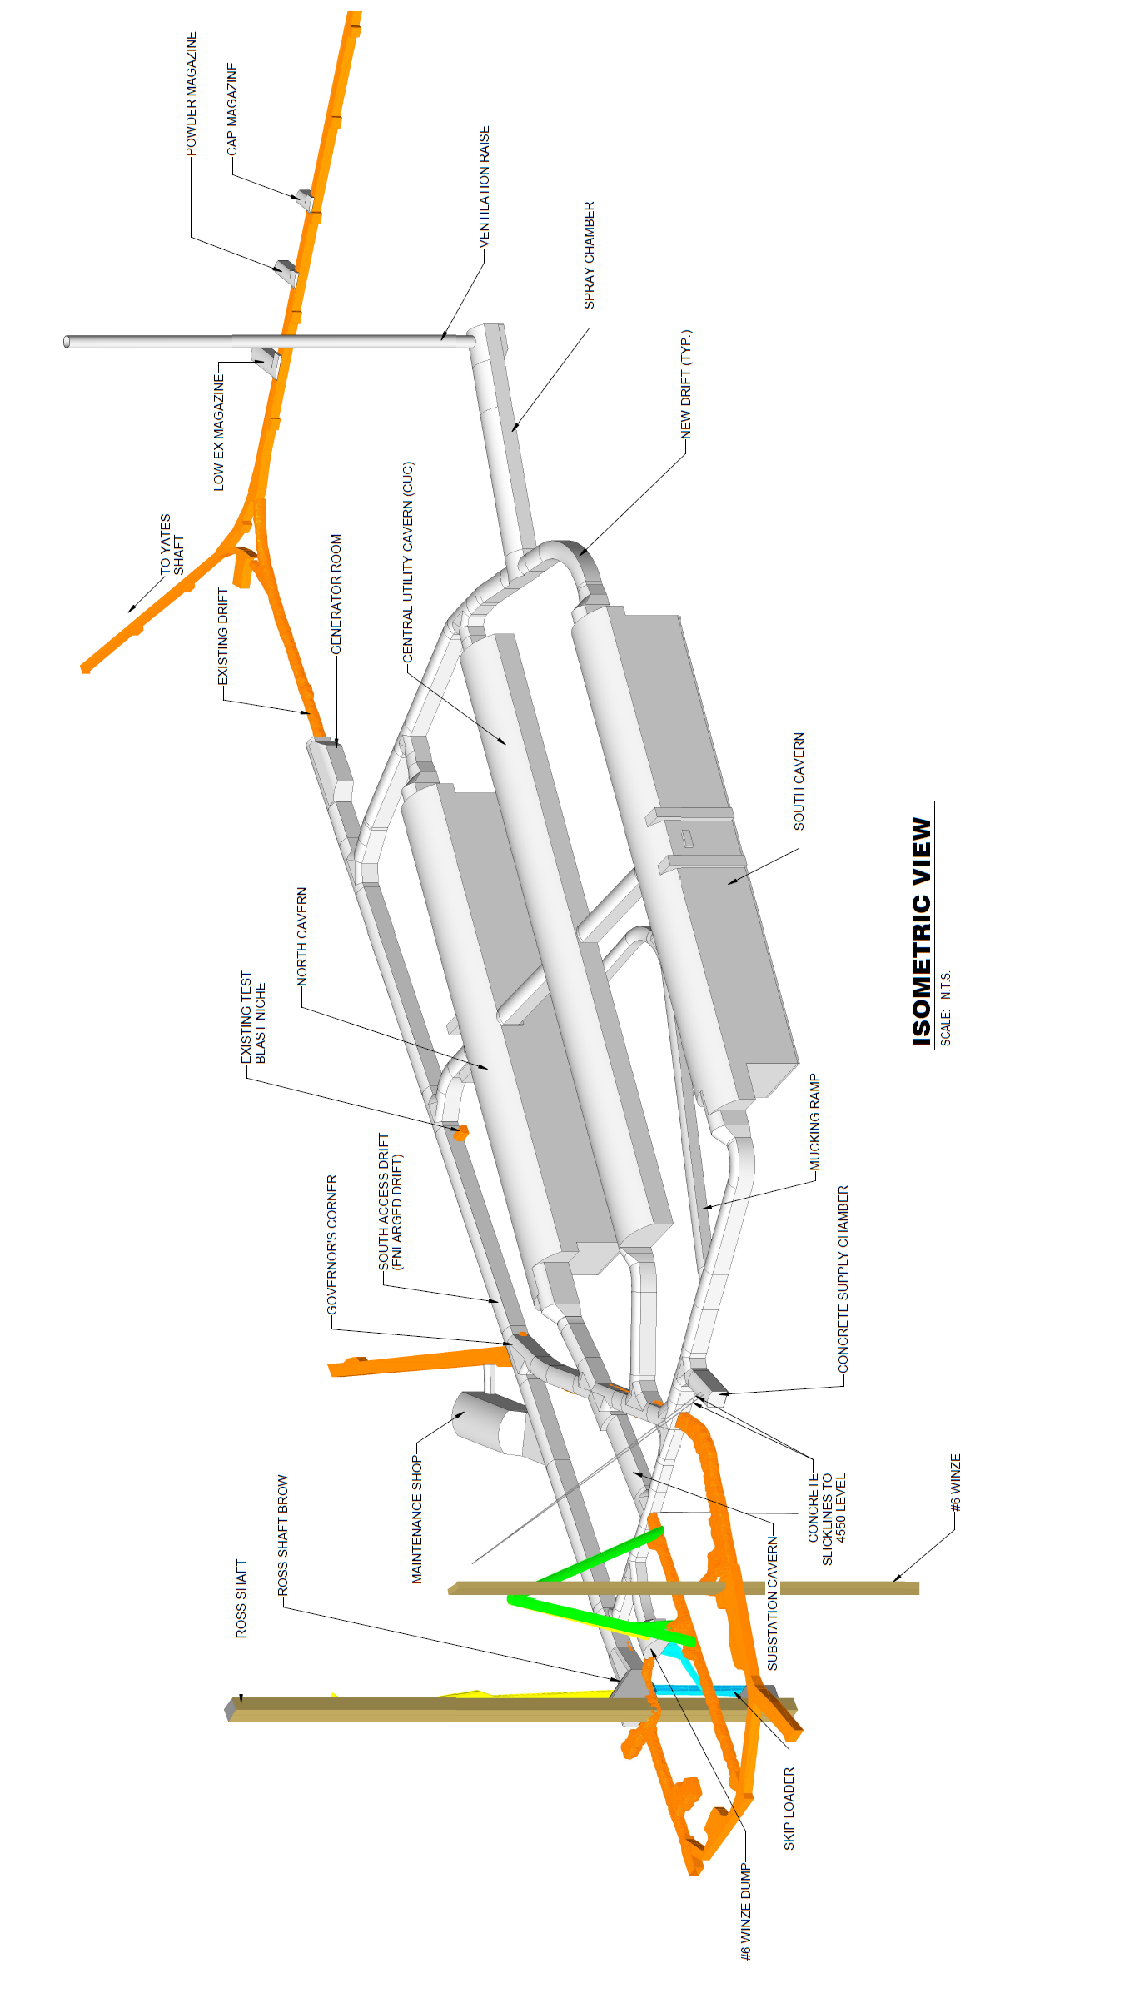
\includegraphics[width=0.75\textwidth]{underground_campus_vertical.pdf}
\end{dunefigure}
\dword{lbnf} will provide facilities and services, on the surface and
underground, to support the \dword{dune} detectors.  This includes
logistical, cryogenic, electrical, mechanical, cyber and environmental
facilities and services.  All of these needed for work at the surface
and underground can be performed and the detectors can be operated in
a safe and productive manner.

The primary path for both personnel and material access to the
underground excavations is through the Ross shaft. On the surface, the
Ross shaft and Ross head frame are undergoing major upgrades. The
structure of the head frame that supports the conveyances is being
reinforced and renovated to make the work flow more efficient and
safer.  All of the wood timber from the 100+ year old shaft has been
removed and replaced with steel sets to improve the time required to
traverse the 4850 L to the underground spaces.  The brakes, drive,
clutches and controls for the conveyance are being completely
overhauled and updated.  In addition to all of these improvements, a
new cage is being designed and fabricated for the Ross shaft.  The new
cage incorporates features to allow the transport of larger items and
includes rigging points underneath for slung loads without the removal
of the cage.  Details on the Ross cage design and size constraints for
material and slung loads can be found in DocDB-3582.

On the surface, a new compressor building is being constructed
adjacent to the head frame.  This building will house the cryogenics
systems for receiving cryogenic fluids and preparing them for delivery
down the Ross shaft.  New piping is being installed down the Ross
shaft compartment to transport cryogens (GAr and N$_2$) underground.

New transformers are being installed in the Ross substation on the
surface to support the underground power needs.  New power cables are
being installed down the Ross shaft to transmit the power underground
to a new substation.

A portion of the Ross Dry basement is being refurbished to house the
surface cyber infrastructure (main communications room --- MCR)
required for data and other underground information.  Redundant fiber
optic cables will leave the MCR to travel down both the Ross and Yates
shafts to newly excavated underground Communication Distribution Room
--- CDR.  From the CDR, the fibers branch out to the \dword{cuc} and detector
caverns to support detector data, cryogenic and detector safety
systems and will be tied into the Building Management System --- BMS.
The BMS controls the facilities Fire and Life Safety --- FLS systems.
All FLS signals from the detector or cryogenic safety systems will be
tied into the facilities BMS for communications to personnel
underground and on the surface.

\section{Detector Caverns}
\label{sec:fdsp-coord-faci-caverns}


Underground spaces are being excavated to support the four
\dword{dune} detectors and infrastructure.  Two large detector caverns
are being excavated.  Each of these caverns will support two
\SI{17}{\kilo\tonne} cryostats.  These caverns, labeled North and
South, are \SI{144.5}{\meter} long, \SI{19.8}{\meter} wide and
\SI{27.95}{\meter} high.  A \SI{12}{\meter} space between the
cryostats will be used as part of the detector installation process,
placement of cryogenic pumps and valves and for access to the 4910
level.  The \dword{cuc}, between the North and South caverns, is
\SI{190}{\meter} long, \SI{19.3}{\meter} wide, and \SI{10.95}{\meter}
high.  The \dword{cuc} will house infrastructure items, such as
cryogenic equipment, Nitrogen dewars and compressors, data acquisition
racks and electronics, chillers for the underground cooling and
electrical services to support the underground space and detectors.
These three main caverns will be connected via a series of drifts as
shown in Figure~\ref{fig:dune-underground}. Access tunnels lie at the
east and west ends of each cavern, north and south side of north
cavern and north side of south cavern. Additionally, the cross section
of the existing drifts where experimental components will be
transported, is being increased to allow passage.  Other ancillary
spaces being provided underground include a maintenance shop,
electrical substation, concrete supply chamber, compressor room, a
spray chamber to house the cooling tower for heat rejection to the
mine air for exhaust through a new 1200 foot$\times$12 foot diameter bore
hole up to the 3650 level.  This bore hole will provide
additional ventilation to support excavation.

Detector one will be built in the east side of the north cavern and
detecor two will be built in the east side of the south cavern. This
is shown in Figure~\ref{fig:dune-full_assmebly}.
\begin{dunefigure}[\dword{dune} cryostat]{fig:dune-full_assmebly}
  {Placement of detector one and two in north and south caverns respectively}
  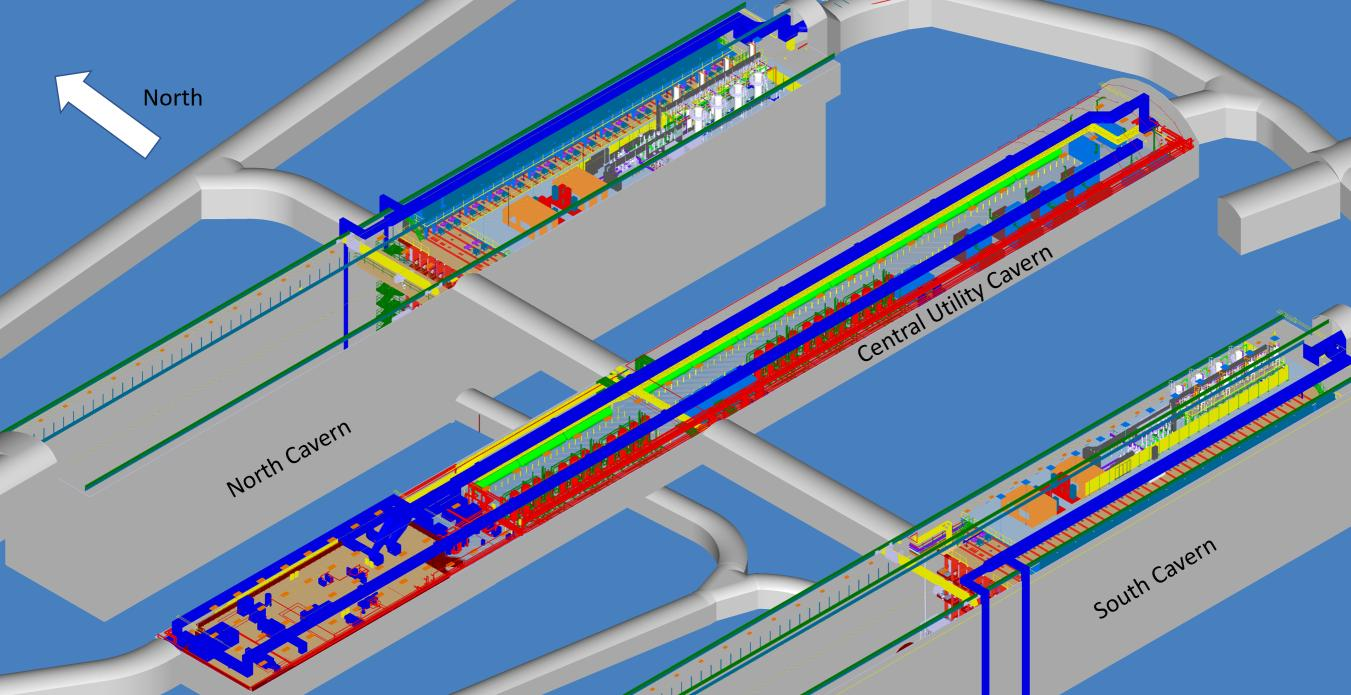
\includegraphics[width=0.85\textwidth]{LBNF_full_assembly.jpg}
\end{dunefigure}
The primary reasons for constructing the first detectors in the east
sides of two caverns are:
\begin{itemize}
\item {\bf Personnel safety during construction and filling}: It is
  planned that detector one will be in the filling phase while detector
  two is in the construction phase. Therefore, construction of the the
  second detector has to take place in a totally separate cavern from
  filling of the first detector. In addition, the airflow in both
  caverns is in the west to east direction. Therefore, construction
  personnel who are primarily on the west side of the detectors will
  be on the upstream side of the airflow.
\item{\bf Access during construction}: The main access for bringing
  large items into both caverns is from the west side. It is,
  therefore, more advantageous that items that enter from the west are
  directly lowered and do not have to pass over detector construction
  site.
\end{itemize}
Both of the reasons above result in the same conclusion that the
detectors one and two are built on the east side of both caverns, and
that they are built in two separate caverns. It is, therefore, planned
that both caverns are ready for beneficial occupancy at the start of
respective detector construction phases.  It should be noted that both
detectors will be built at the 4910 level. However, with the exception
of the LAr circulation pumps, all services are at the 4850 level.

To support the electrical requirements new XX kVA power feeds will be
routed from the surface substation down the Ross shaft to the
underground electrical substation and from the substation to the
electrical room in the \dword{cuc}.  The electrical room will have multiple
transformers from which to distribute power for various functions such
as lighting, HVAC, cryogenic equipment and detector power.  Each
detector cavern and the DAQ room will have dedicated feeds from the
electrical room.  Details of this are described in the electrical
section.  There are multiple electrical panels planned in each cavern
to provide power for the different phases of construction.  These
phases would include the installation of the cryostat warm structure
and cold membrane, detector installation and detector
operations. During detector operations separate panels are available
for detector (clean) and building (dirty) power.

To support underground cooling requirements, four 400-ton chillers
will be located in the \dword{cuc} adjacent to the electrical room and
cryogenics equipment.  These chillers are designed to provide \SI{400}{\kilo\watt}
of cooling for the various cryogenic systems, 500 kW of cooling for
the electronics on each of the detectors and 750 kW of cooling to the
DAQ room in the \dword{cuc}.  These chillers will also provide chilled water
to the HVAC systems underground to maintain the ambient temperature
and humidity.

Fire protection in the underground spaces will be determined by zone,
hazard type and requirements.  Details of this can be found on ARUP
drawing U1-FD-E-651 in the Underground Electrical package and is shown
in Figure~\ref{fig:lbnf-fire}
\begin{dunefigure}[Underground fire zones]{fig:lbnf-fire}
  {Underground fire zones}
 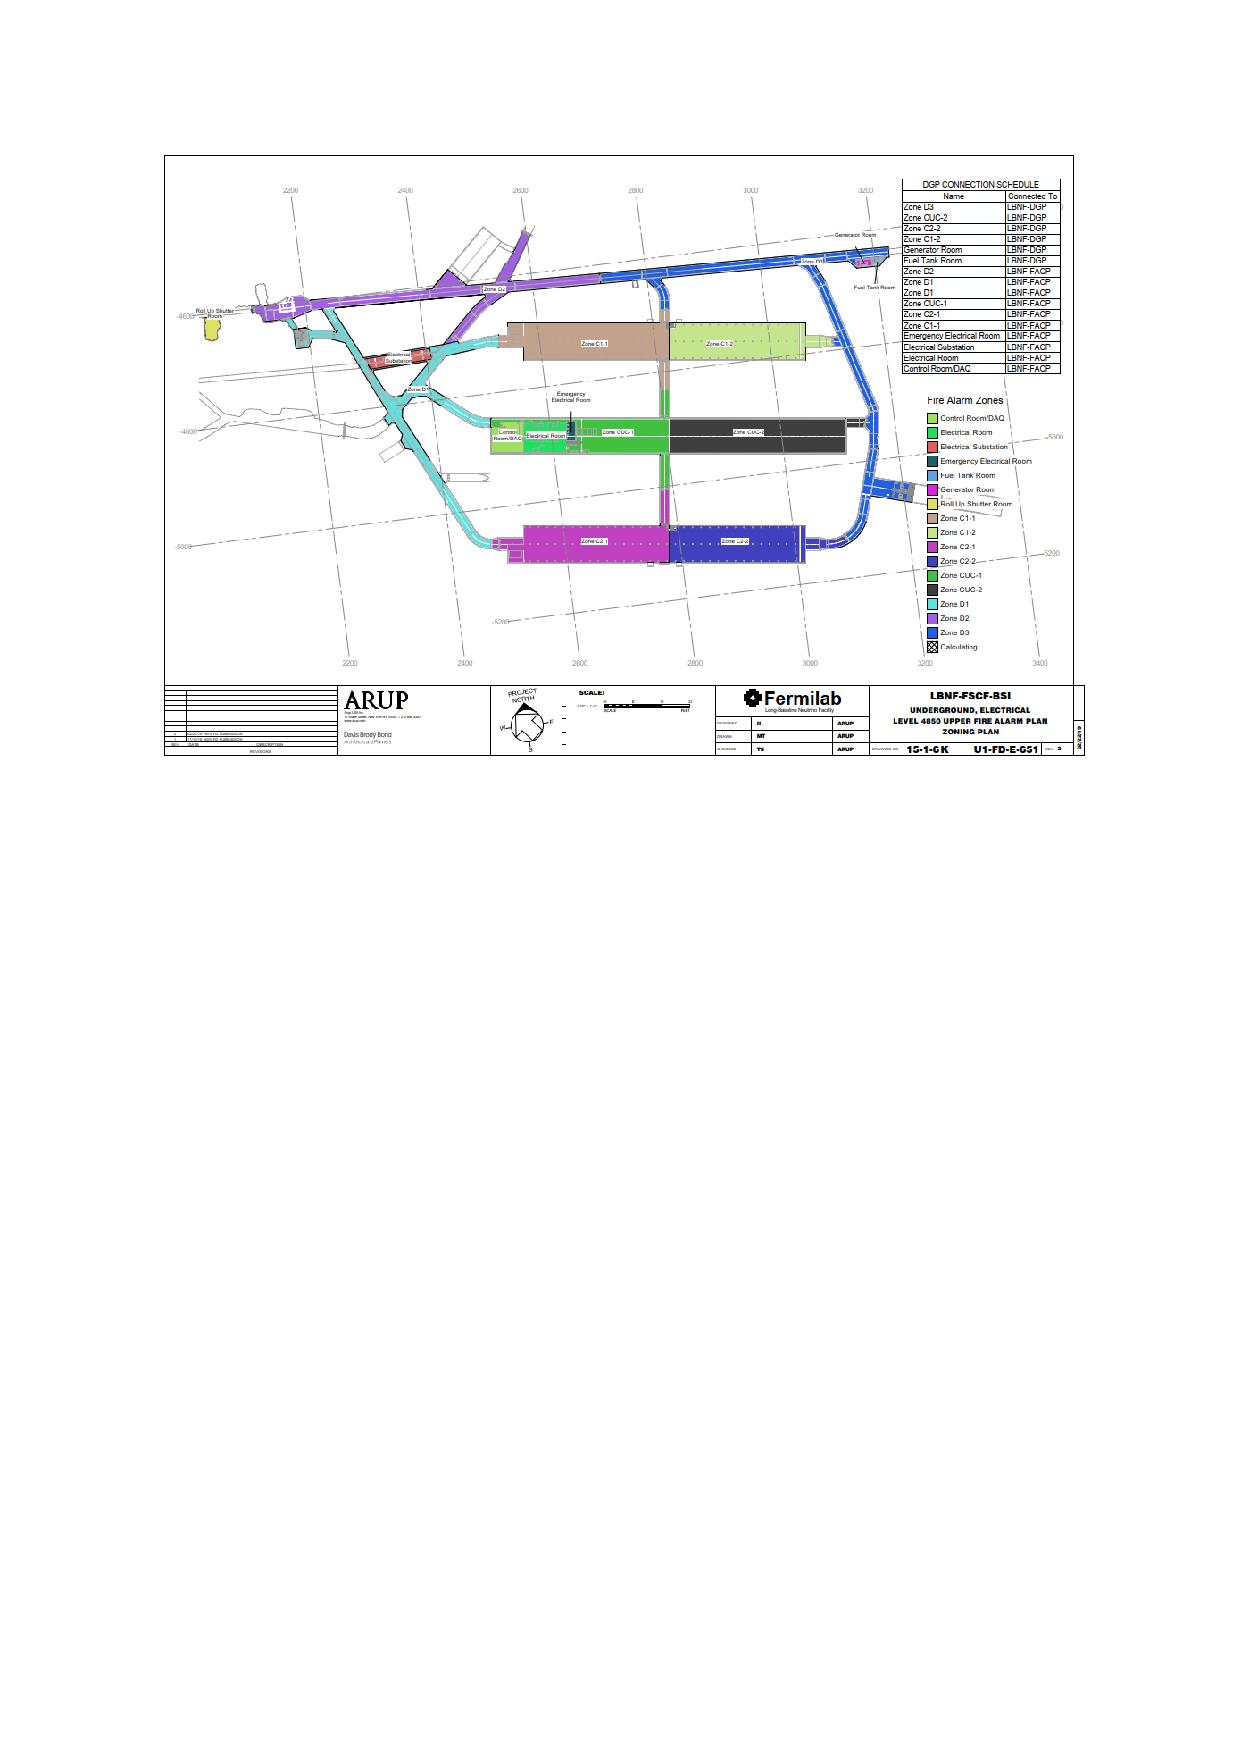
\includegraphics[width=0.85\textwidth]{lbnf_fire}
\end{dunefigure}
The drifts will be outfitted with normal wet type sprinklers and
broken into three zones.  The North and South caverns will be outfitted
with a pre-action type sprinkler system to protect sensitive detector
electronics from water damage from accidental release.  A pre-action
system requires two signals to activate.  These are the detection of
smoke from the by one of the sensors and the fusing of the sprinkler
head.  This type of system was the most economic choice to lessen the
risk of unnecessary discharge of water over the detector electronics.
The DDSS will interface with the BMS fire system to turn off the power
to the racks before water would be introduced to lessen the impact of
the water on the system and reduce the risk of electrical shock.  A
pre-action system will also be installed in the CUC over the cryogenic
equipment as shown in the figure.  In the electrical substation,
electrical room, DAQ room and CDR, a clean agent type system will be
employed.  Clean agent systems use either inert gas or chemical agents
to extinguish a fire and are typically used in areas that contain
sensitive electronics or data/power centers.

In addition to the above services, systems are being installed to
provide compressed air, industrial water, internet and a configurable
security access system.

\section{Cryostat}
\label{sec:fdsp-coord-cryostat}

Each detector will be housed inside a cryostat designed to hold the
liquid argon (LAr), cryogenic piping and the detector as shown in
Figure~\ref{fig:dune-cryostat}.
\begin{dunefigure}[\dword{dune} cryostat]{fig:dune-cryostat}
  {Overall construction and dimensions of the \dword{dune} cryostat.}
  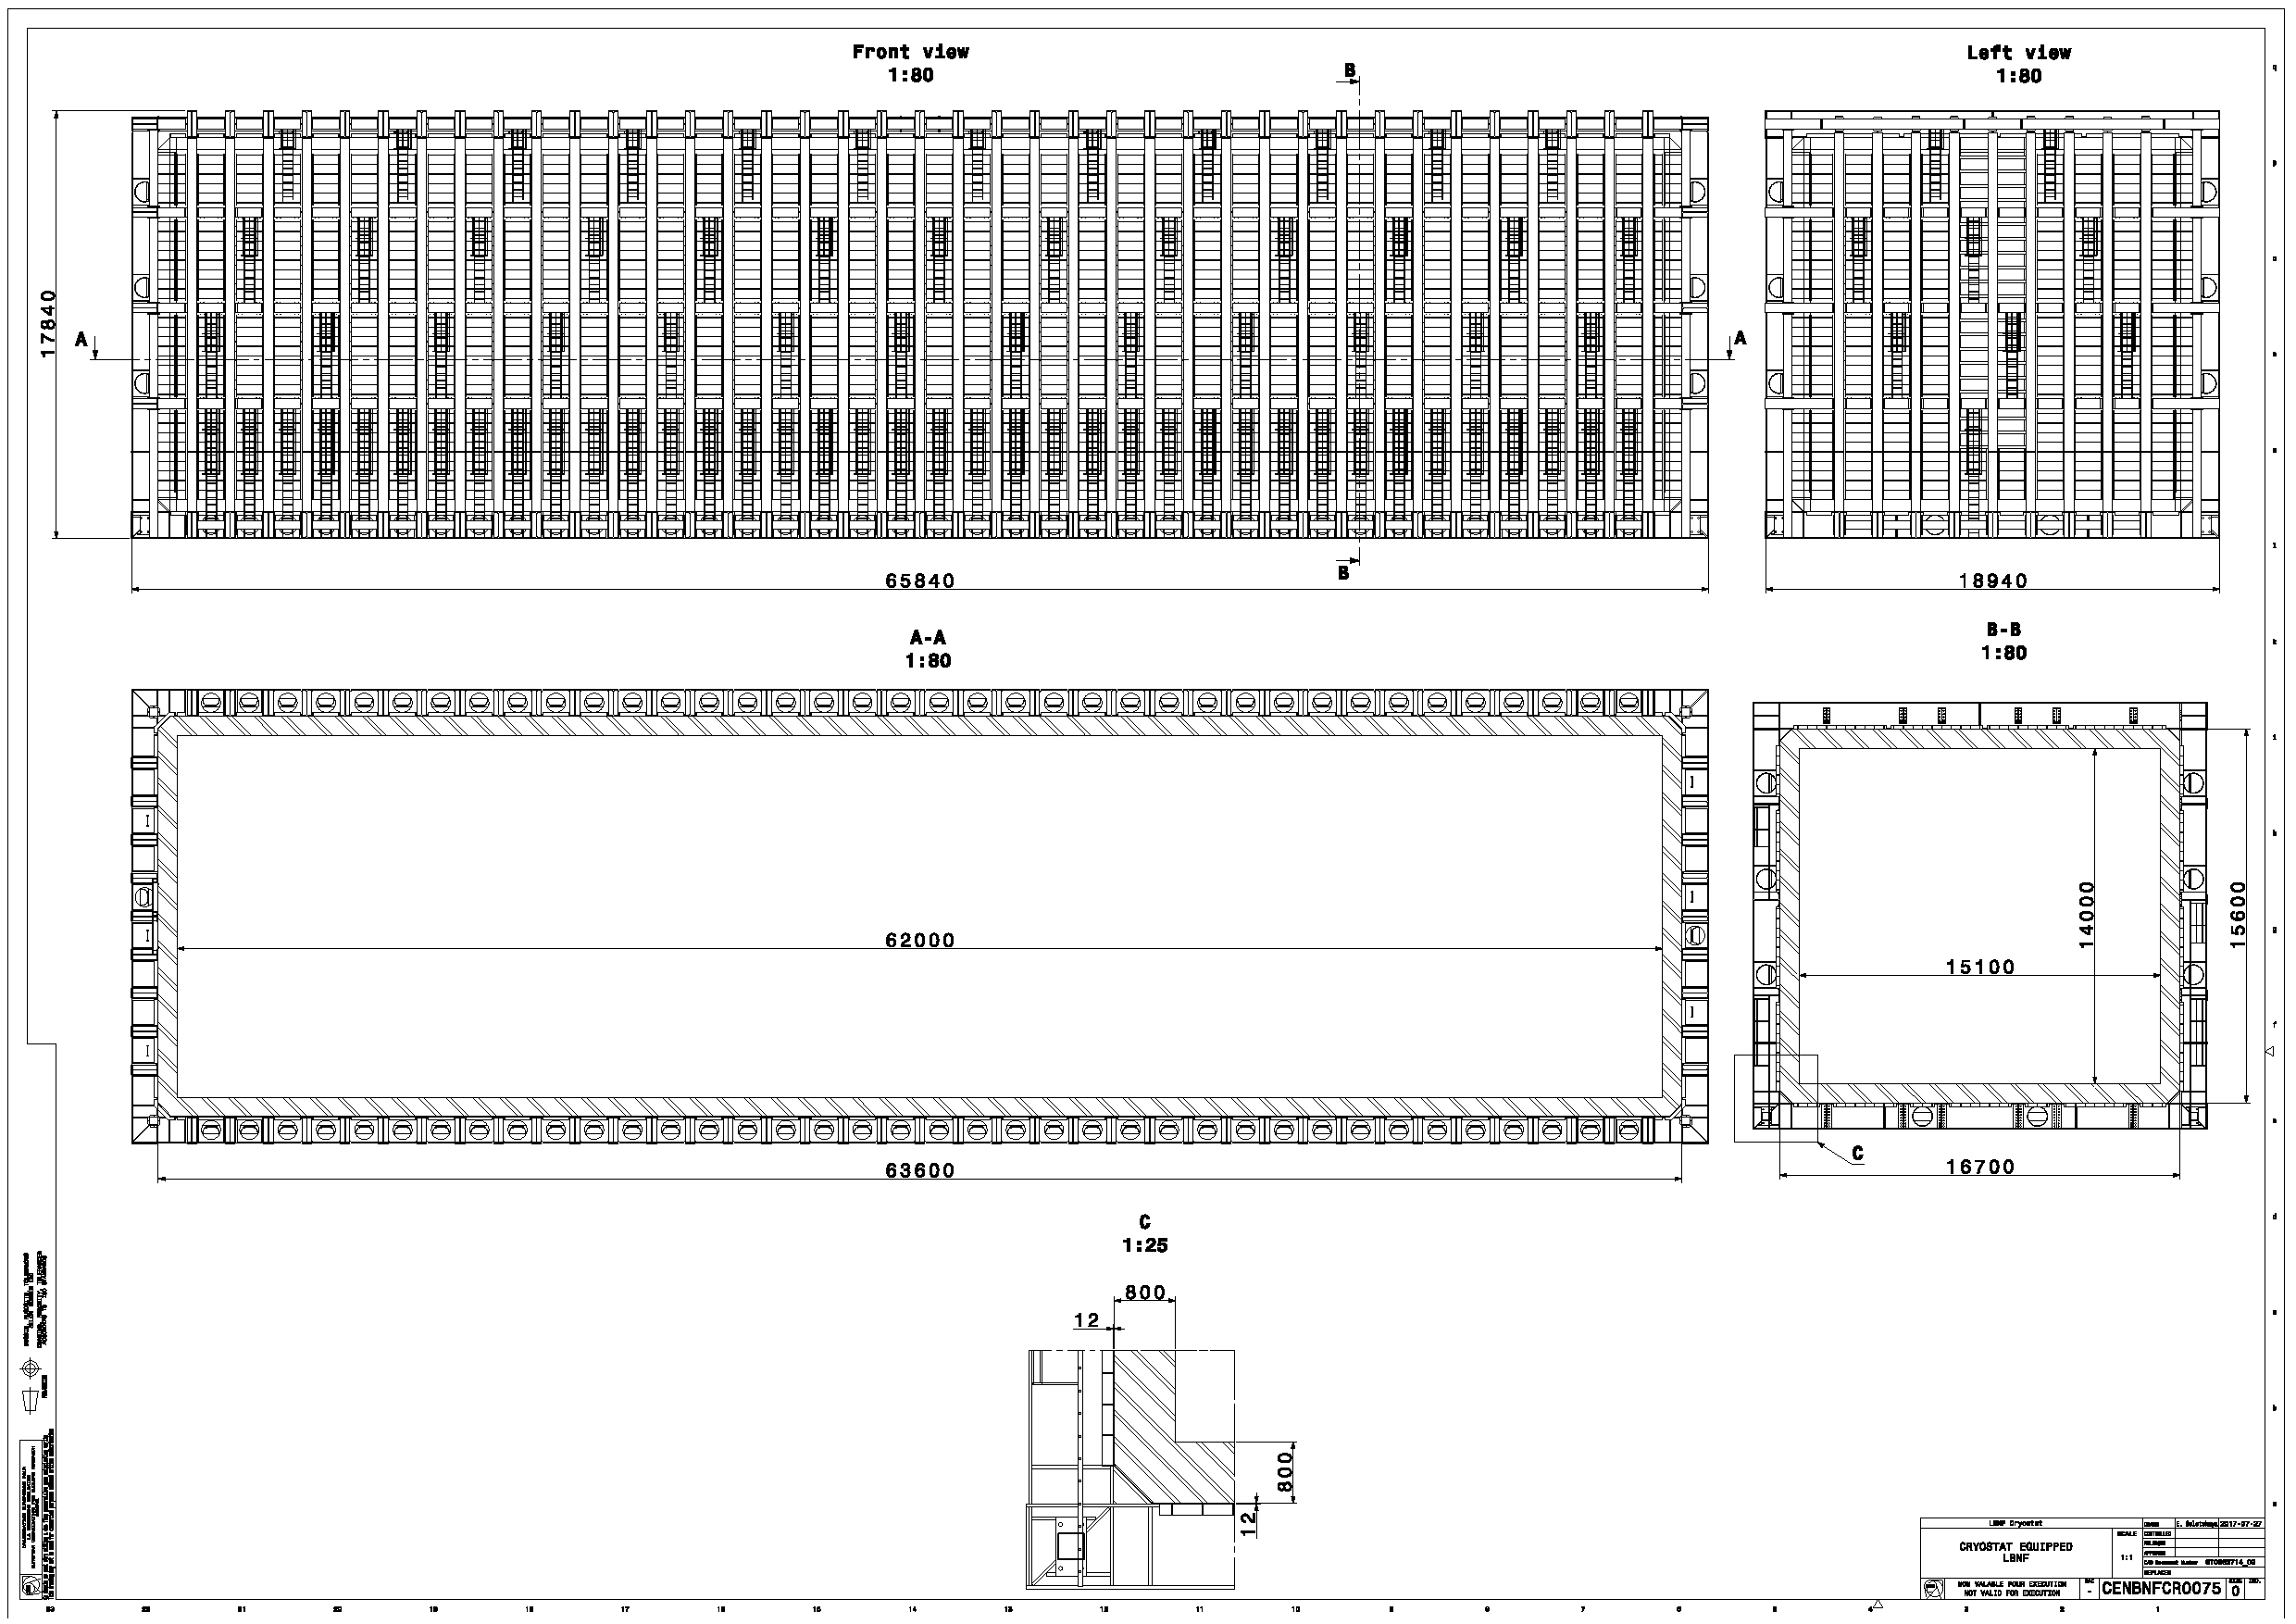
\includegraphics[width=0.85\textwidth]{cryostat.pdf}
\end{dunefigure}
Each cryostat consists of a warm structure that provides structural
support, insulating layers that maintain the temperature of the fluid
inside and the inner membrane that provides a compliant inner surface
that helps to maintain the LAr purity and serves as primary
containment.

The warm structure measures \SI{65.84}{\meter} long,
\SI{18.94}{\meter} wide and \SI{17.84}{\meter} high externally and
\SI{63.6}{\meter} long, \SI{16.7}{\meter} wide and \SI{15.6}{\meter}
high internally.  It is a welded and bolted structure constructed of
I-beam elements and a \SI{12}{\mm} inner steel plate reinforced with
ribs.  It is designed support the self-weight of the structure,
insulation, inner membrane, liquid, detector and any equipment placed
on the structure.  It also supports the hydrostatic pressure of the
fluid inside and resists the small gas overpressure in the ullage.
The structure is positioned on the concrete slab provided at the 4910L
of the North and South caverns.  The 12 mm inner steel plate of the
warm structure also serves as the tertiary layer of containment.

The insulation layer and inner membrane will be installed inside the
warm structure.  The technology for this comes from the shipping
vessels used for transporting liquid natural gas. The insulating
layers are made from prefabricated panels of reinforced polyurethane
foam.  There are two layers of the foam panels that have a flexible
membrane in between that serves as a secondary containment membrane.
The two foam layers are installed in an overlapping pattern to reduce
heat introduced into the fluid.  The total thickness of the two foam
layers is \SI{0.8}{\meter} with a density of approximately
\SI{90}{mg/cm$^3$} and a residual heat input of
\SI{6.3}{W/\meter$^2$}.  A stainless steel corrugated membrane will be
installed inside the insulating layers to create the primary
containment membrane for the LAr.  This is constructed from < 2 mm
thick stainless steel panels that overlap and are welded together.
The entire inner surface of the cryostat will be tiled with these
panels to create the inner surface.  These panels need to be
corrugated to accommodate the shrinkage of the stainless steel from
ambient temperature to LAr temperature.  With the addition of the
insulation and inner membrane, the internal dimensions of the finished
vessel are \SI{62}{\meter} long, \SI{15.1}{\meter} wide and
\SI{14}{\meter} high.

The top of the cryostat will have penetrations provided based on
drawings developed by LBNF and DUNE to accommodate detector support,
electronic and data cables, cryogenic pipes and connections and other
devices.

Each cryostat will have a vertical \dword{tco} on one short end.
These openings will be approximately \SI{13.43}{\meter} high and
\SI{2.68}{\meter} wide and will be used to move the detector elements
into the vessel during installation.  Once most of the detector
material is inside the cryostat, the \dword{tco} will be closed and
leak tested.  After the \dword{tco} closing, the last of the detector
installation will be completed. After final detector installation and
equipment removal through the roof openings, the cryostat will be
closed for purge, cooldown and filling.

At the \dword{tco} end of the cryostat, there will be four penetrations for
the cryogenic fluid pumps to be connected.  A normally closed valve
will be installed at each penetration to prevent any loss of fluid
with pump maintenance or damage.

\section{Cryogenics}
\label{sec:fdsp-coord-cryogenics}


The detector cryogenics system supplies \dword{lar} and provides
circulation, re-condensation and purification. The cryogenic system
components are housed inside the \dword{cuc}, on top of each detector module
and between the two detector modules in each cavern. The cryogenic system comprises
\begin{itemize}
\item {\bf Infrastructure Cryogenics}: This includes \dword{lar} and LN$_2$ receiving
  facilities on the surface, nitrogen refrigeration systems (both
  above ground and underground), LN$_2$ buffer storage
  underground, piping to interconnect equipment (LN$_2$, GN$_2$ and GAr),
  components in the detector cavern and the \dword{cuc} and process control/support
  equipment.
\item {\bf Proximity cryogenics}: This includes reliquefaction 
  and purification subsystems for the argon (both gas and liquid), associated
  instrumentation and monitoring equipment and \dword{lar} piping to
  interconnect equipment and components in the detector cavern and the
  \dword{cuc}. The proximity cryogenics are split into three areas: in the
  \dword{cuc}, on top of the mezzanine, as shown in Figure~\ref{fig:detector_mezzanines},
  and on the side of the cryostat where \dword{lar} circulation pumps are installed.
\item {\bf Internal cryogenics}: This includes \dword{lar} and GAr distribution
  systems inside the cryostat, as well as features to cool the
  cryostat and the detector uniformly.
\end{itemize}

Figure~\ref{fig:dune-cryogenics} shows the process flow diagram of the
\dword{lbnf} cryogenic system. For convenience, only one cryostat is shown. The three main areas are:
\begin{enumerate}
  \item Surface (on the left), with the receiving facilities and the
    recycle compressors of the Nitrogen System.  All these items are
    part of the infrastructure cryogenics.
  \item Central Utility Cavern (in the center), with the LAr/GAr
    purification and regeneration systems (part of the Proximity
    Cryogenics) and the cold boxes, expanders and LN2 storage (part of
    the Infrastructure cryogenics).
\item Detector Cavern (on the right), with the Argon condensing system
  and the distribution of Argon from the purification system in the
  CUC to the cryostat and vice versa.
\end{enumerate}

Argon and Nitrogen are received and stored on the surface in the
liquid phase.  They are vaporized and transferred underground in the
gas phase, the nitrogen as part of the nitrogen system, the argon on
its own. Figure~\ref{fig:dune-cryogenics} shows the process flow
diagram for the cryogenics.
\begin{dunefigure}[Cryogenics system]{fig:dune-cryogenics}
  {Overall process flow diagram of the cryogenic system showing one
    cryostat only; other cryostats are the same.}
  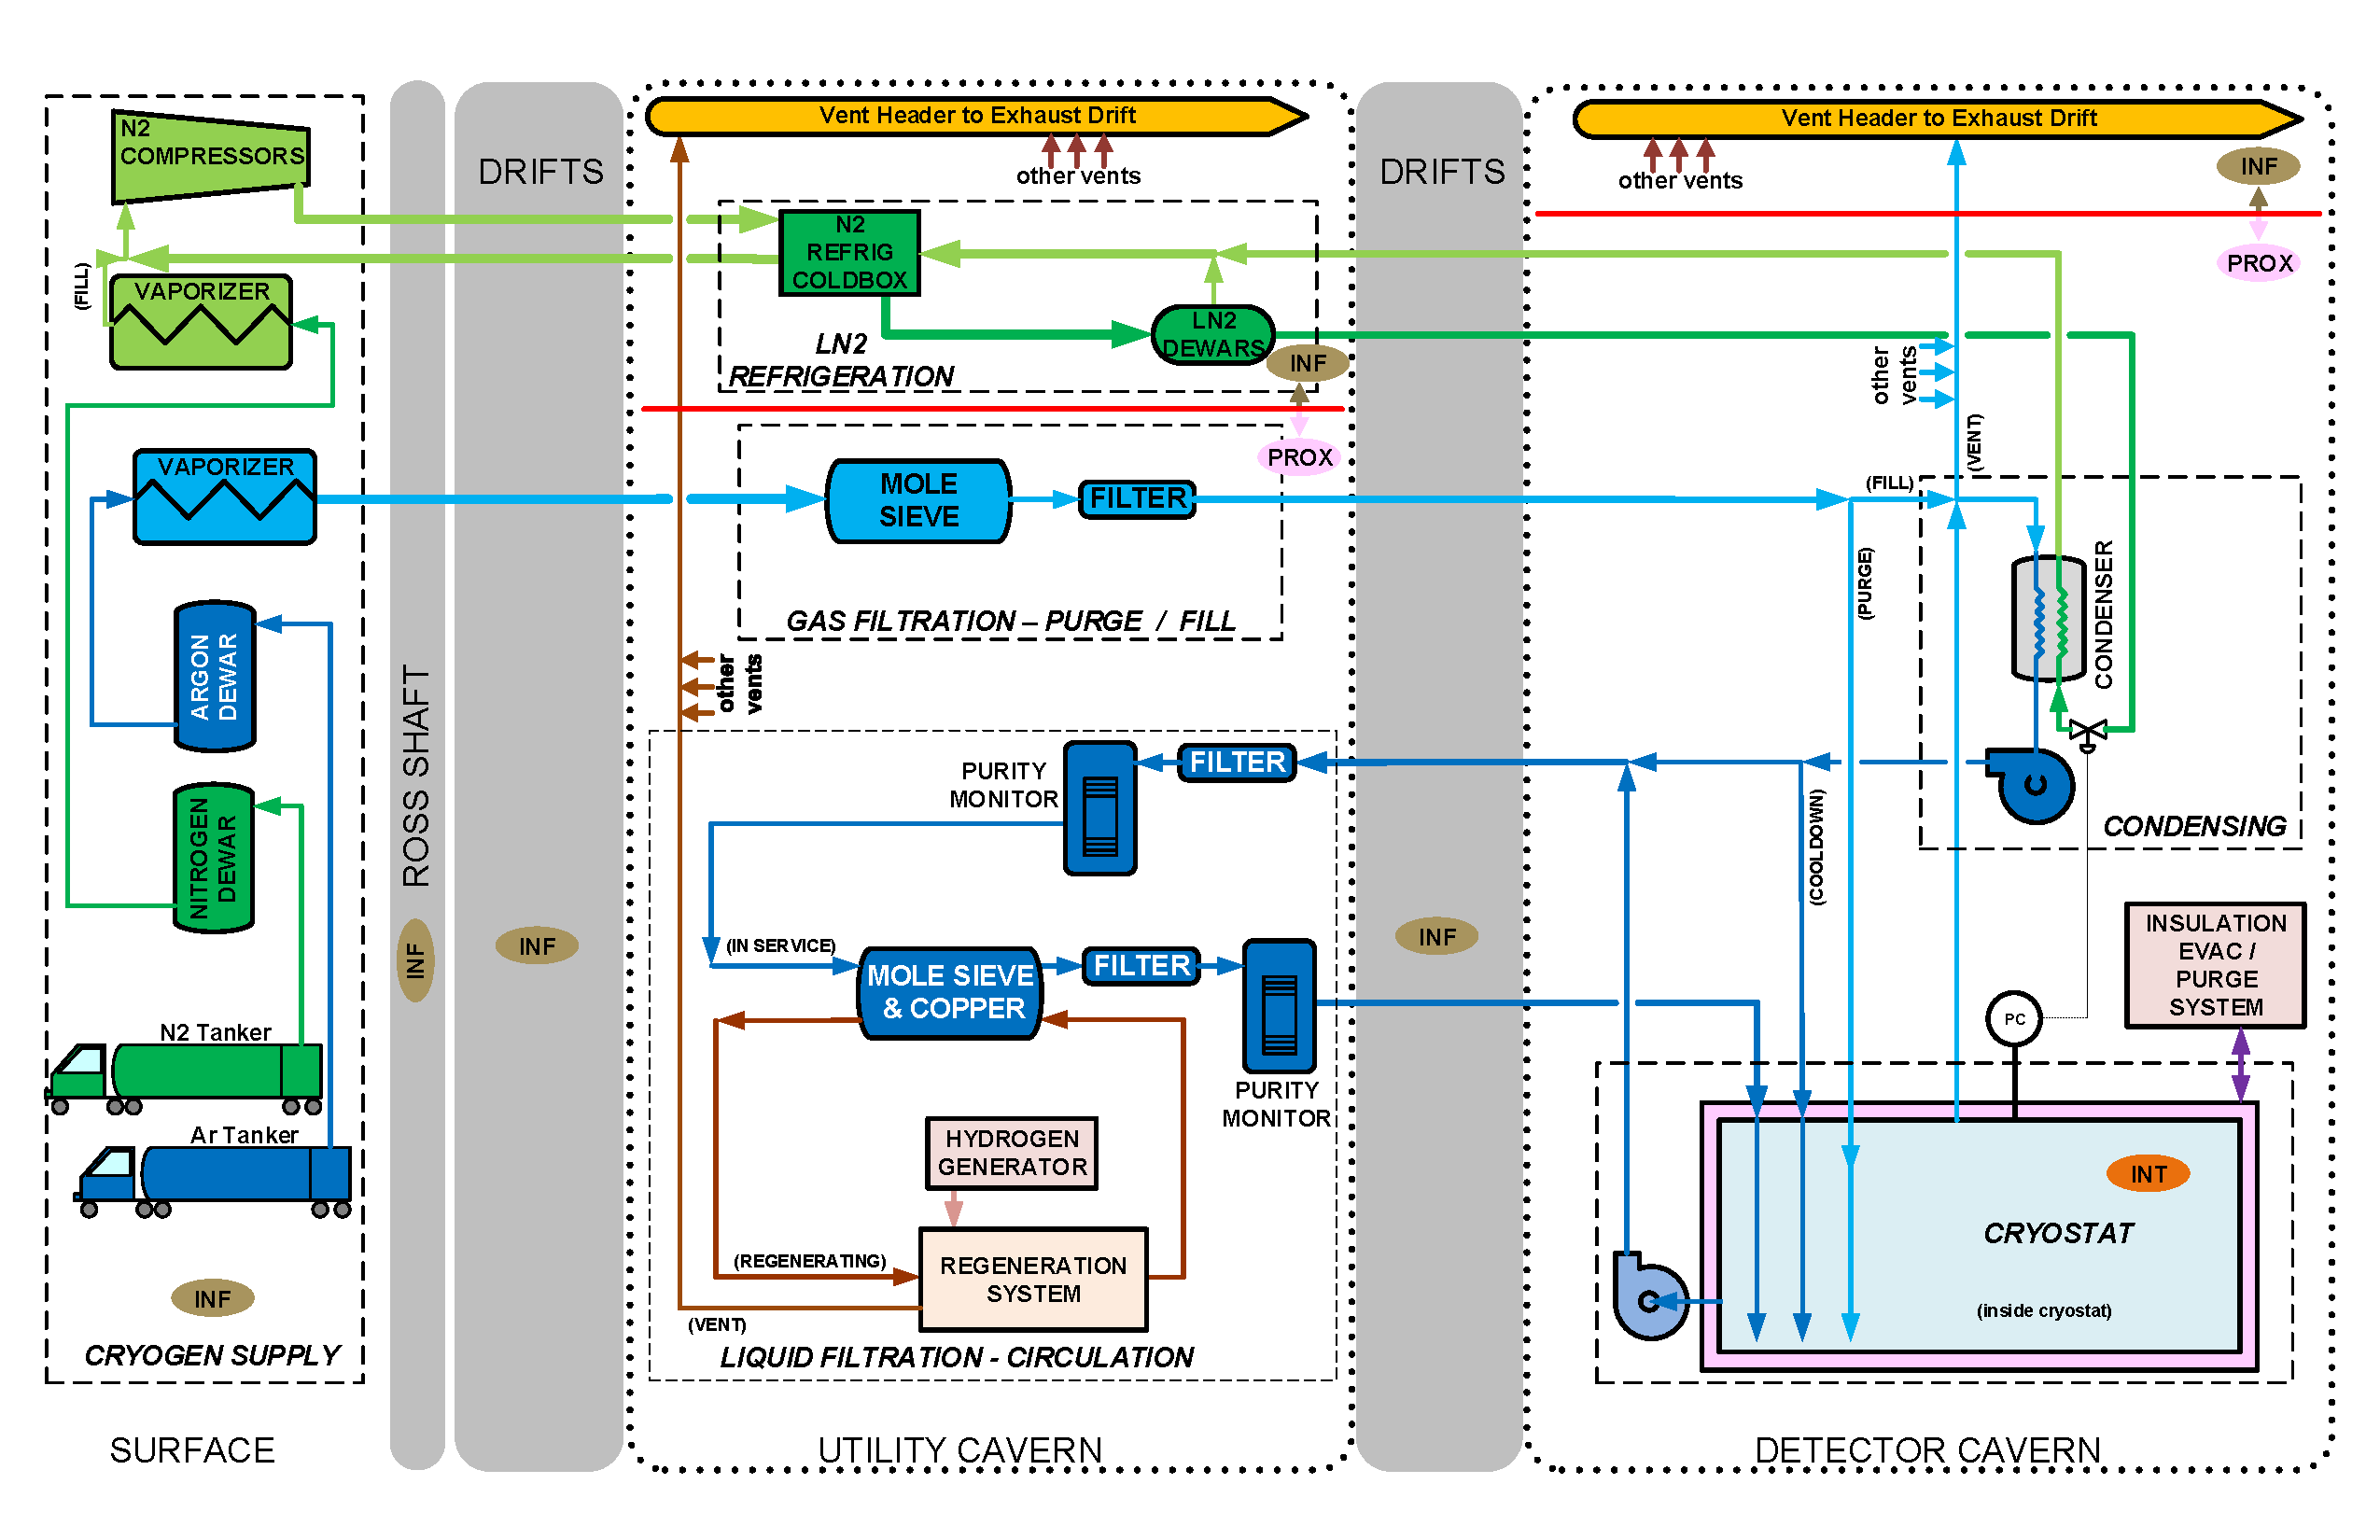
\includegraphics[width=0.85\textwidth]{LBNF_PFD_180909.pdf}
\end{dunefigure}


The cryogenics system fulfills the following modes of operations:
\begin{itemize}
  \item {\bf Gaseous argon purge}: Initially, each cryostat is filled
    with air, which must be removed by means of a slow GAr ``piston
    purge''.  A slow flow of argon is introduced from the bottom and
    displaces the air by pushing it to the top of the cryostat where
    it is vented.  Once the impurities, primarily nitrogen, oxygen,
    water, drop below the parts per million (ppm) level, the argon
    exhausted at the top of the cryostat is circulated in closed loop
    through the gas purification system and re-injected at the
    bottom. Once the contaminants drop below the ppm level, the
    cool-down can commence. The GAr for the purge comes directly from
    above ground, passes through the GAr purification and then it is
    injected at the bottom of the cryostat by means of a GAr
    distribution system.
  \item {\bf Cryostat and detector cool-down}: The detector elements
    must be cooled in a controlled and uniform manner. Purified LAr is
    flown into sprayers that atomize it. A second set of sprayers
    flowing purified GAr moves the mist of argon around to achieve a
    uniform cooling. The cooling power required to recondense argon in
    the condensers outside the cryostat is supplied by the
    vaporization of nitrogen from the nitrogen system. Once the
    detector elements reach about 90 K, the filling can commence. The
    GAr for the cool-down comes directly from above ground, passes
    through the GAr purification and then it is condensed in the
    condensers before being injected in the sprayers. The GAr moving
    the mist of argon around only goes through the GAr purification
    and not the condensers.
  \item {\bf Cryostat filling}:Argon is vaporized and transferred
    underground as a gas from the receiving facilities on the surface.
    It first flows through the GAr purification system and is
    recondensed in the argon condensers by means of vaporization of
    LN2.  It then flows through the LAr purification and is introduced
    in the cryostat. The filling of each cryostat varies in duration,
    from 8 to 15 months, depending on the available cooling power at
    each stage.
  \item{\bf Steady state operations}: The LAr contained inside each
    cryostat is continuously purified through the LAr purification
    system using the main external LAr circulation pumps. The boil-off
    GAr is recondensed in the argon condensers and purified as liquid
    in the same LAr purification system as the bulk of the LAr.
  \item{\bf Cryostat emptying}: At the conclusion of the experiment,
    each cryostat is emptied and the LAr is removed from the system.
\end{itemize}
The process controls are redundant and reside locally in each
chamber. PLC racks are located on the mezzanine, in the pit over the
protective structure of the main LAr circulation pump, in the CUC and
on the surface. A workspace and a desk with two stations are available
on top of the mezzanine and in the CUC respectively for installation
and commissioning.

Before Argon is offloaded from each truck into the receiving tanks, a
sample of the LAr is analyzed locally to ensure compliance with the
requirements. If the specifications are met, the truck driver is given
green light to offload the truck. The process is automated to reduce
human error. The purity is measured before and after the purification
system by custom made purity monitors to verify the correct
functioning of the system.


\section{Detector and Cavern Integration}
\label{sec:fdsp-coord-det-cav-integ}
In this section, integration of the detector modules in the cavern is
shown in following figures and explanations.

Figure~\ref{fig:detector_ew_elevation} shows the north
elevation view of the detector in the cavern. The services from the
\dword{cuc} enter the cavern through a passage visible on the left.
\begin{dunefigure}[North elevation view of Detector]{fig:detector_ew_elevation}
  {North elevation view of one detector module in the cavern.}
  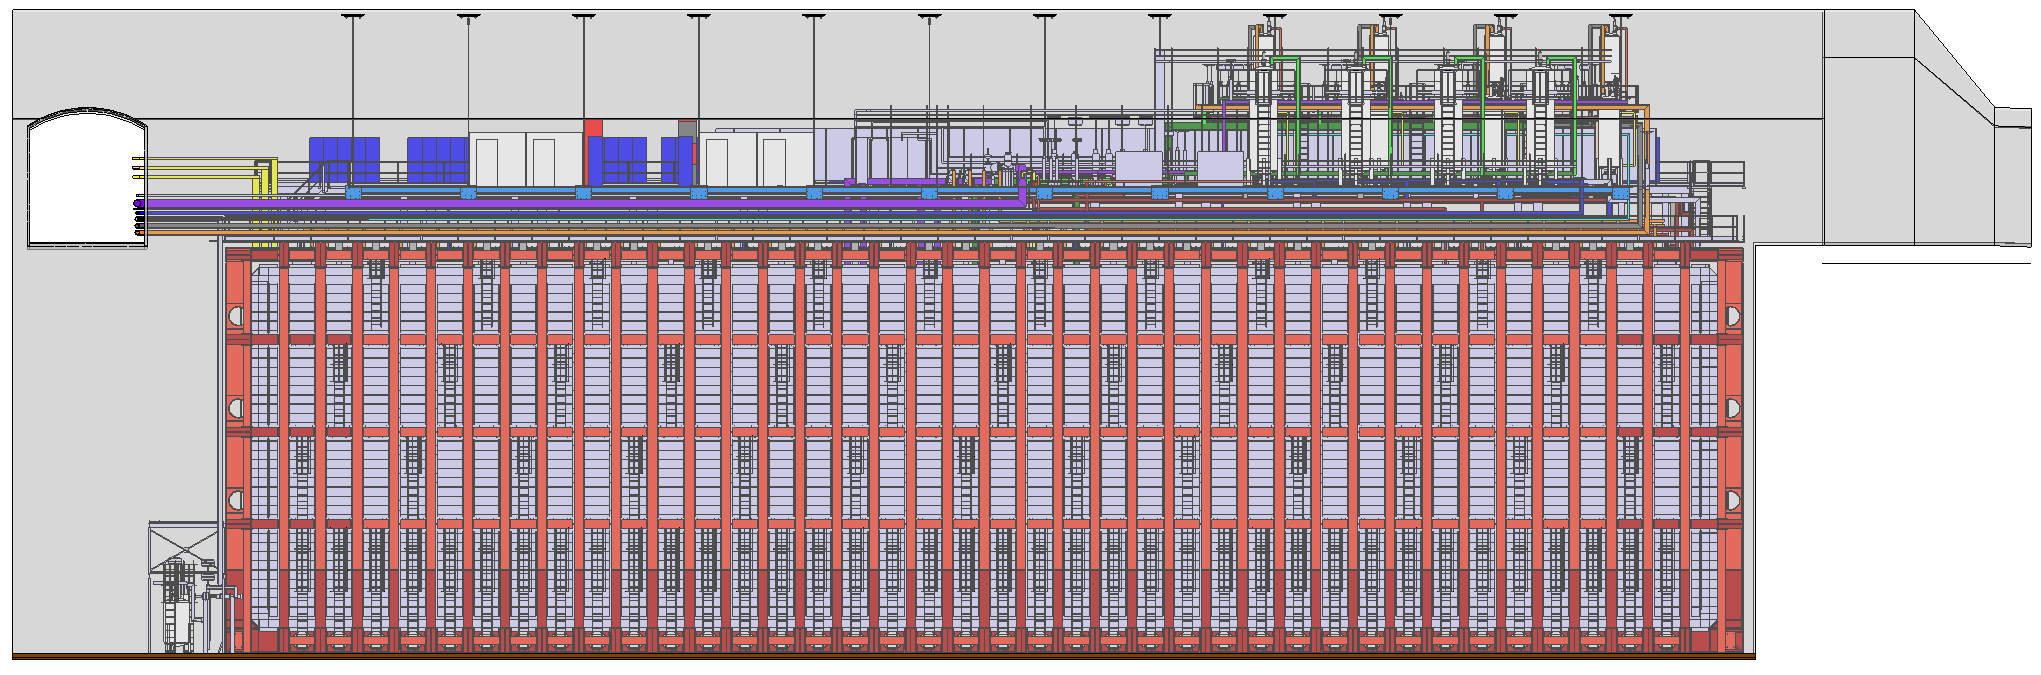
\includegraphics[width=0.75\textwidth]{LBNF-Cryostat-South_Elevation_in_Cavern_c.png}
\end{dunefigure}

Figure~\ref{fig:detector_cavern} shows one detector module in the
cavern. In this figure, the cryogenics equipment and racks on top of
the detector are visible. The \dword{lar} recirculation pumps can also be seen
on the lower level.
\begin{dunefigure}[Overall view of the detector in cavern.]{fig:detector_cavern}
  {Overall view of a detector module within the cavern.}
  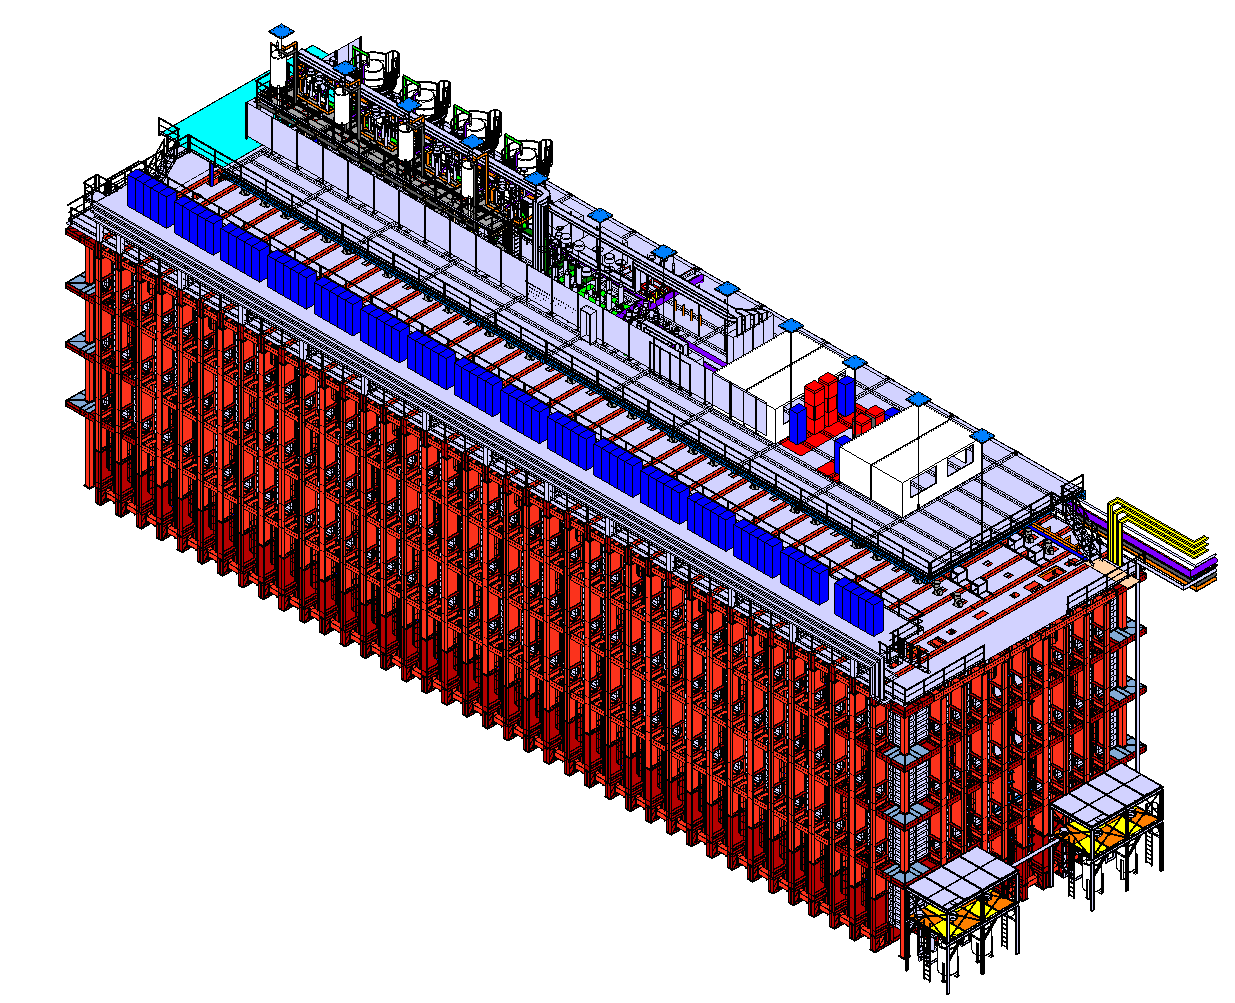
\includegraphics[width=0.8\textwidth]{LBNF-Cryostat-NW_Iso_c.png}
\end{dunefigure}

Figure~\ref{fig:detector_ns_elevation} shows the west
elevation view of the detector in the cavern. The services entering
from the \dword{cuc} are visible on the right.
\begin{dunefigure}[West elevation view of detector]{fig:detector_ns_elevation}
  {West elevation view of one detector in the cavernwith overall dimensions.}
  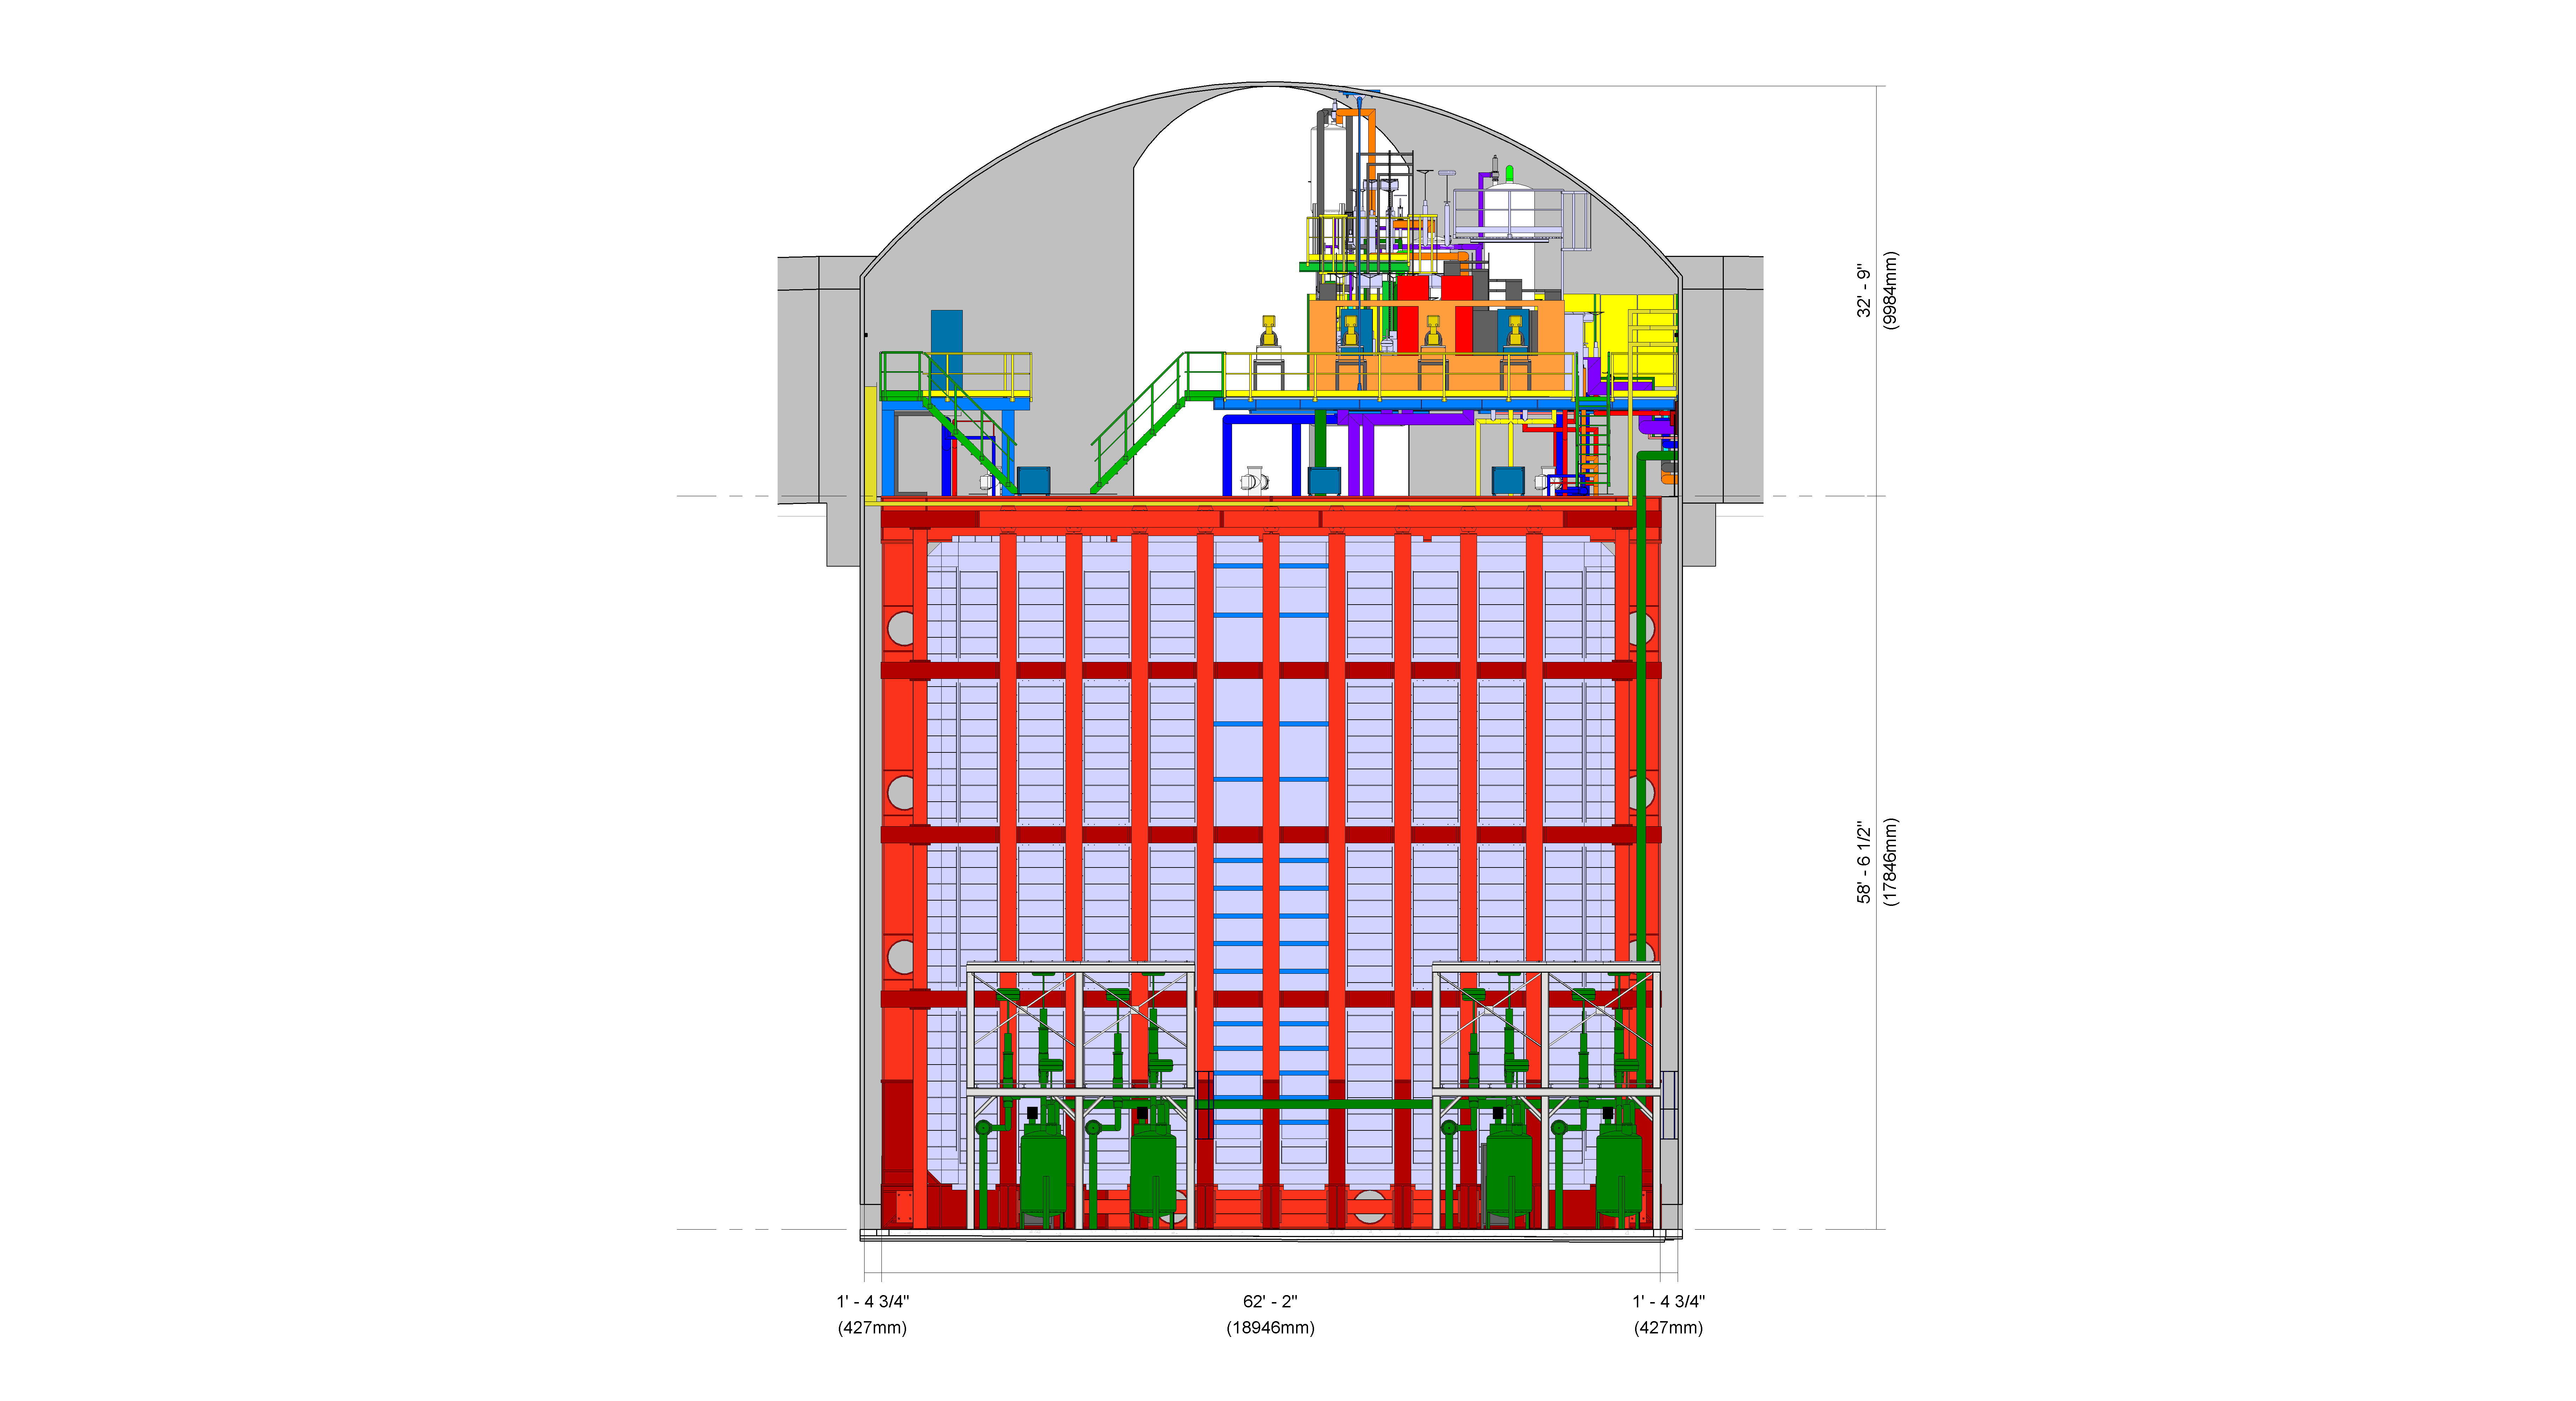
\includegraphics[width=0.9\textwidth]{LBNF-Cryostat-West_Elevation_in_Cavern_c_with_Dimensions.png}
\end{dunefigure}

Figure~\ref{fig:detector_mezzanines} shows the elevation view of the
top of cryostat showing mezzanines, cryogenic equipment, and
electronic racks.
\begin{dunefigure}[Elevation view of top of cryostat showing mezzanines, cryogenic
    equipment and electronic racks.]{fig:detector_mezzanines}
  {Elevation view of top of cryostat showing mezzanines, cryogenic
    equipment, and electronic racks.}
  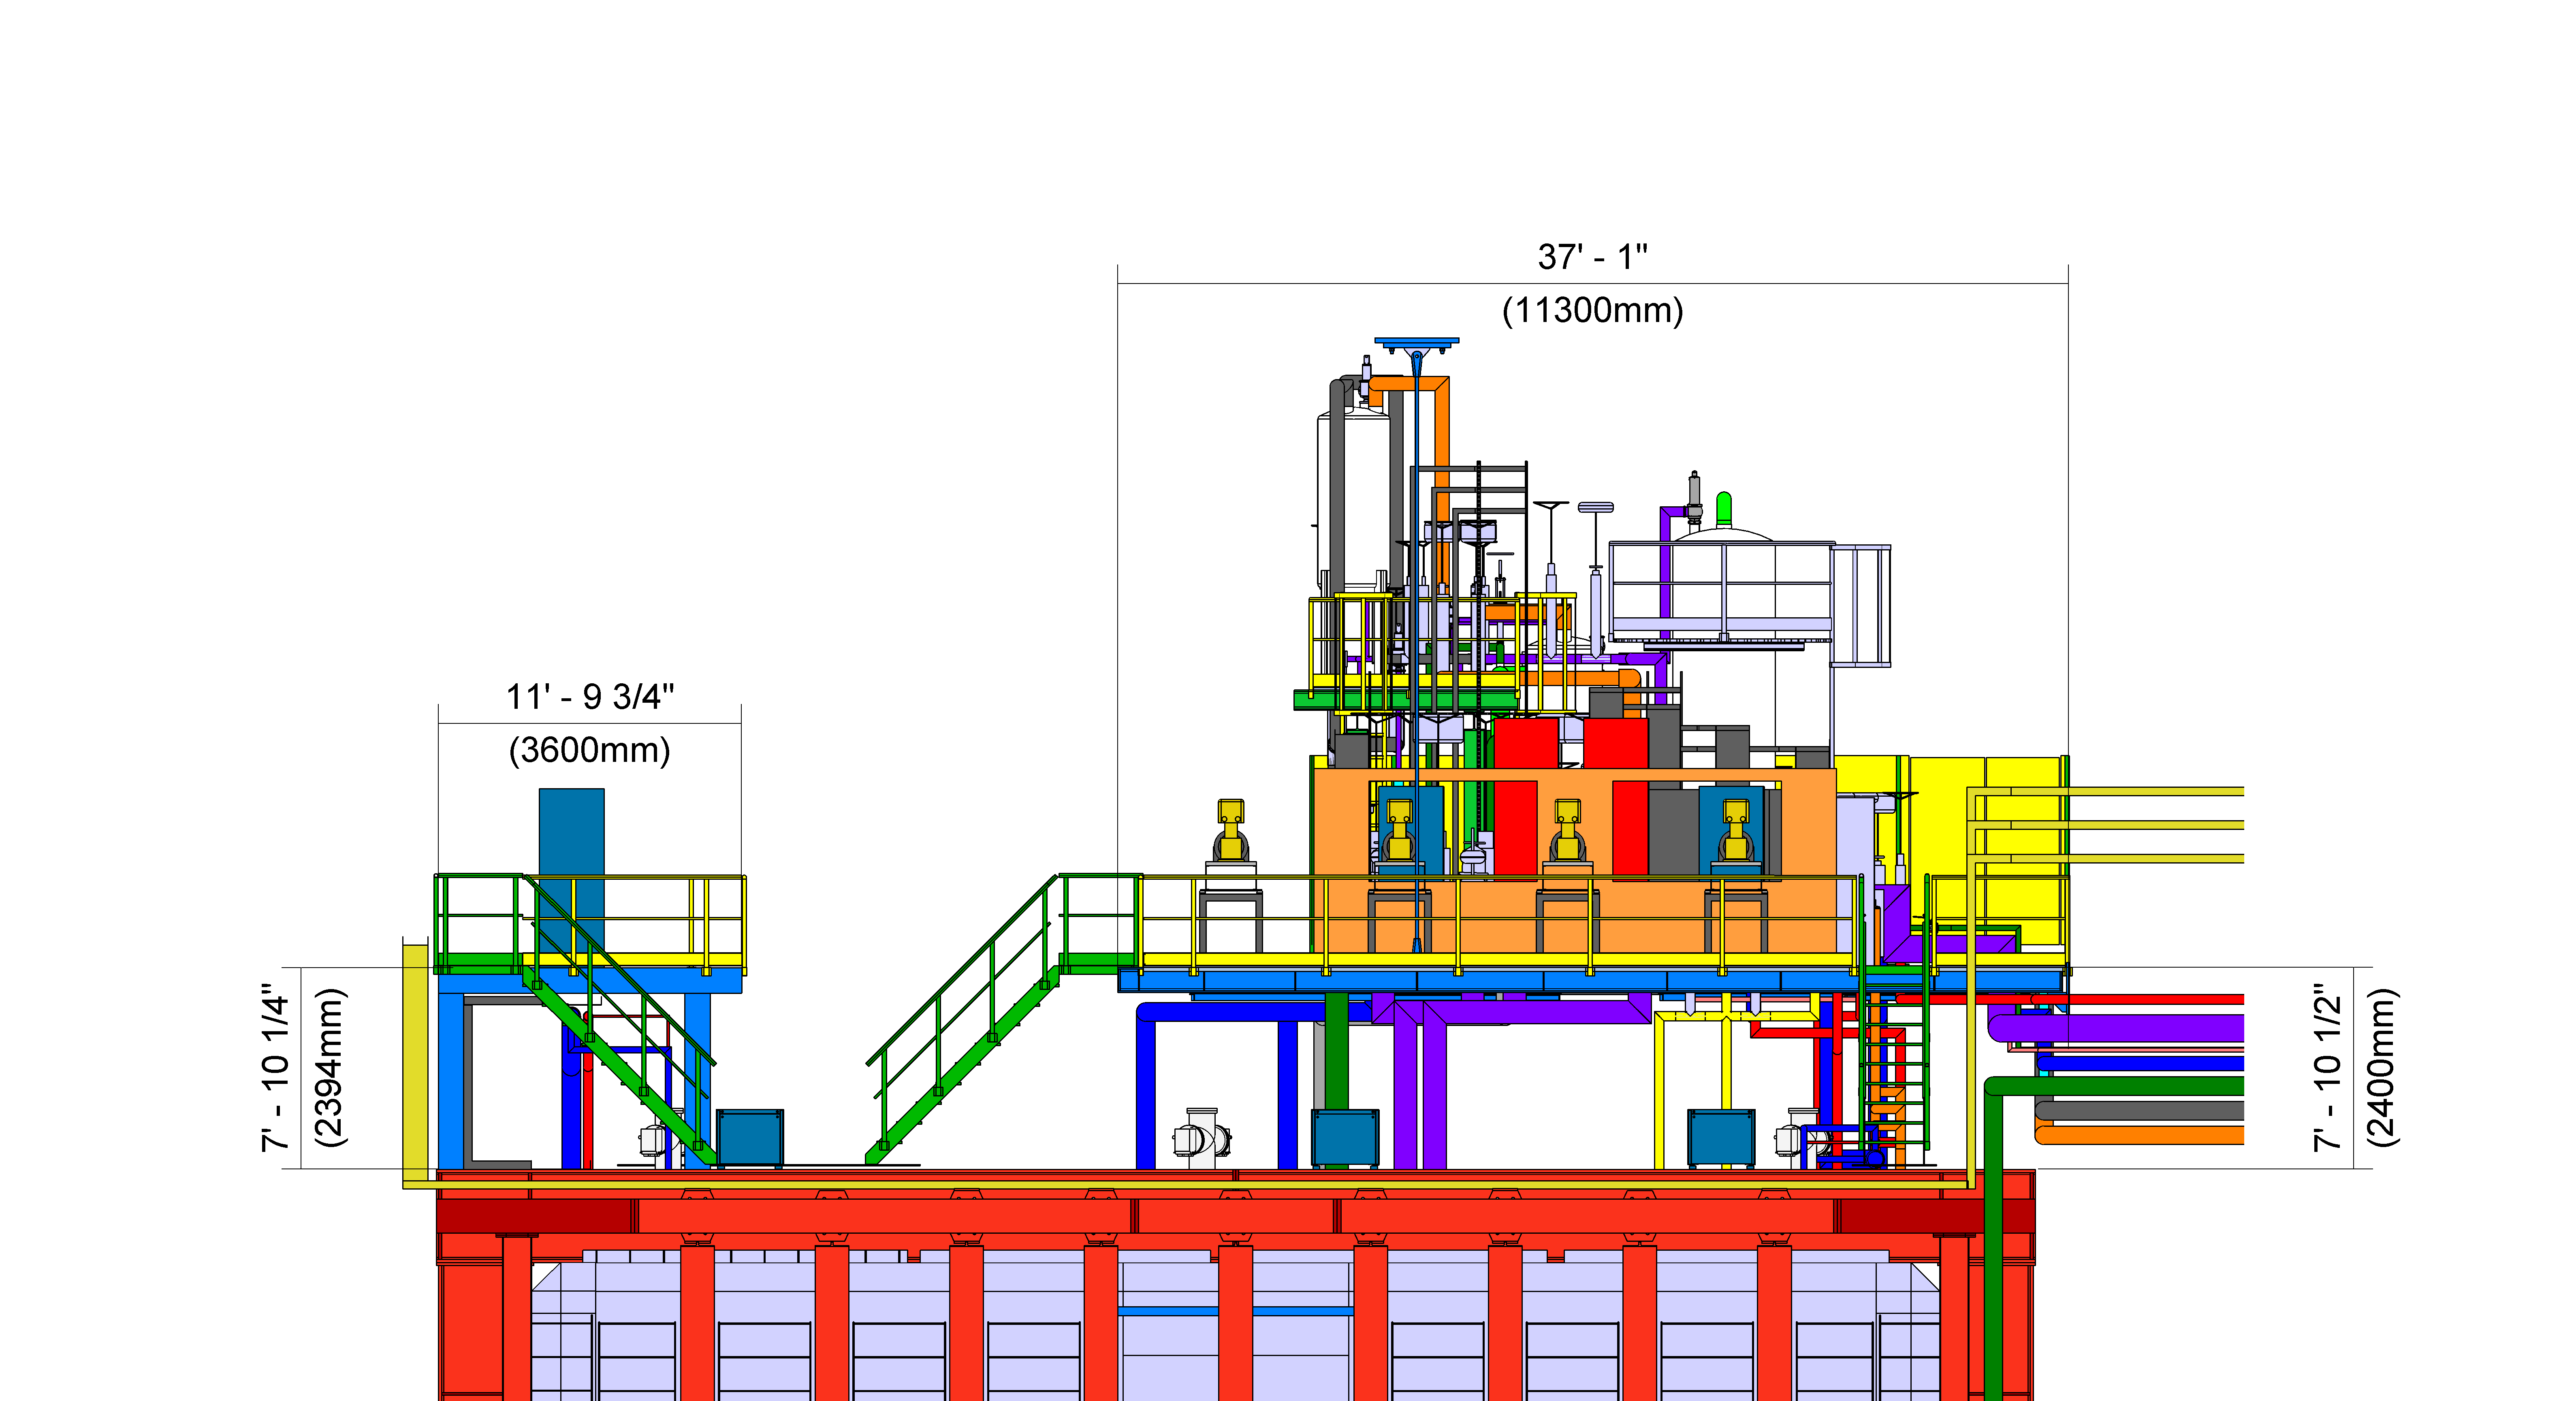
\includegraphics[width=0.85\textwidth]{LBNF-Cryostat-West_Elevation-Cryo_c_with_Dimensions.png}
\end{dunefigure}
The cryogenics are installed on a mezzanine supported from
the cavern roof and cavern wall. Cryogenic distribution lines are
routed under the mezzanine. Local control rooms for the
cryogenic equipment are on the mezzanine.

Detector electronics are installed in short racks close to
feedthroughs and in taller racks installed on a separate electronics
mezzanine shown on the left of Fig.~\ref{fig:detector_mezzanines}.
This will allow easy access for maintenance and reduce complexity on
top of the detector.

\section{Detector Grounding}
\label{sec:fdsp-coord-faci-grounding}


The grounding strategy provides the detectors with independent
isolated grounds to minimize any environmental electrical noise that
could couple into detector readout electronics either conductively or
through emitted electromagnetic interference.

The detectors will be placed at the 4910 level of \surf. The
electrical conductivity of the various rock masses are unknown but
should have extremely poor and inconsistent conductive
properties. Ensuring adequate sensitivity of the detectors requires a
special ground system that will isolate the detectors from all other
electrical systems and equipment, minimize the influence of inductive
and capacitive coupling, and eliminate ground loops. The grounding
infrastructure should reduce or eliminate ground currents through the
detector that would affect detector sensitivity, maintain a low
impedance current path for equipment short circuit and ground fault
currents, and ensure personnel safety by limiting any potential for
equipment-to-equipment and equipment-to-ground contact.

The infrastructure grounding plan of the underground facilities is
fully described in EDMS 2095975.  The plan is to have a separate
Detector Ground for each of the four detectors which is isolated from
the rest of the facility.  The Detector Ground will primarily be
comprised of the steel containment vessel, cryostat membrane and
connected readout electronics.  The facility ground is constructed out
of two interconnected grounding structures; these are the Cavern
Ground and the Ufer Grounds which are described below.  For safety
reasons, a saturable inductor will connect the Detector Ground to the
rest of the facility.

Figure~\ref{fig:dune-grounding} shows the areas of construction for
the Cavern and Ufer grounds.
\begin{dunefigure}[Overall \dword{dune} grounding structure]{fig:dune-grounding}
  {Overall \dword{dune} facility grounding structure incorporated in cavern.}
  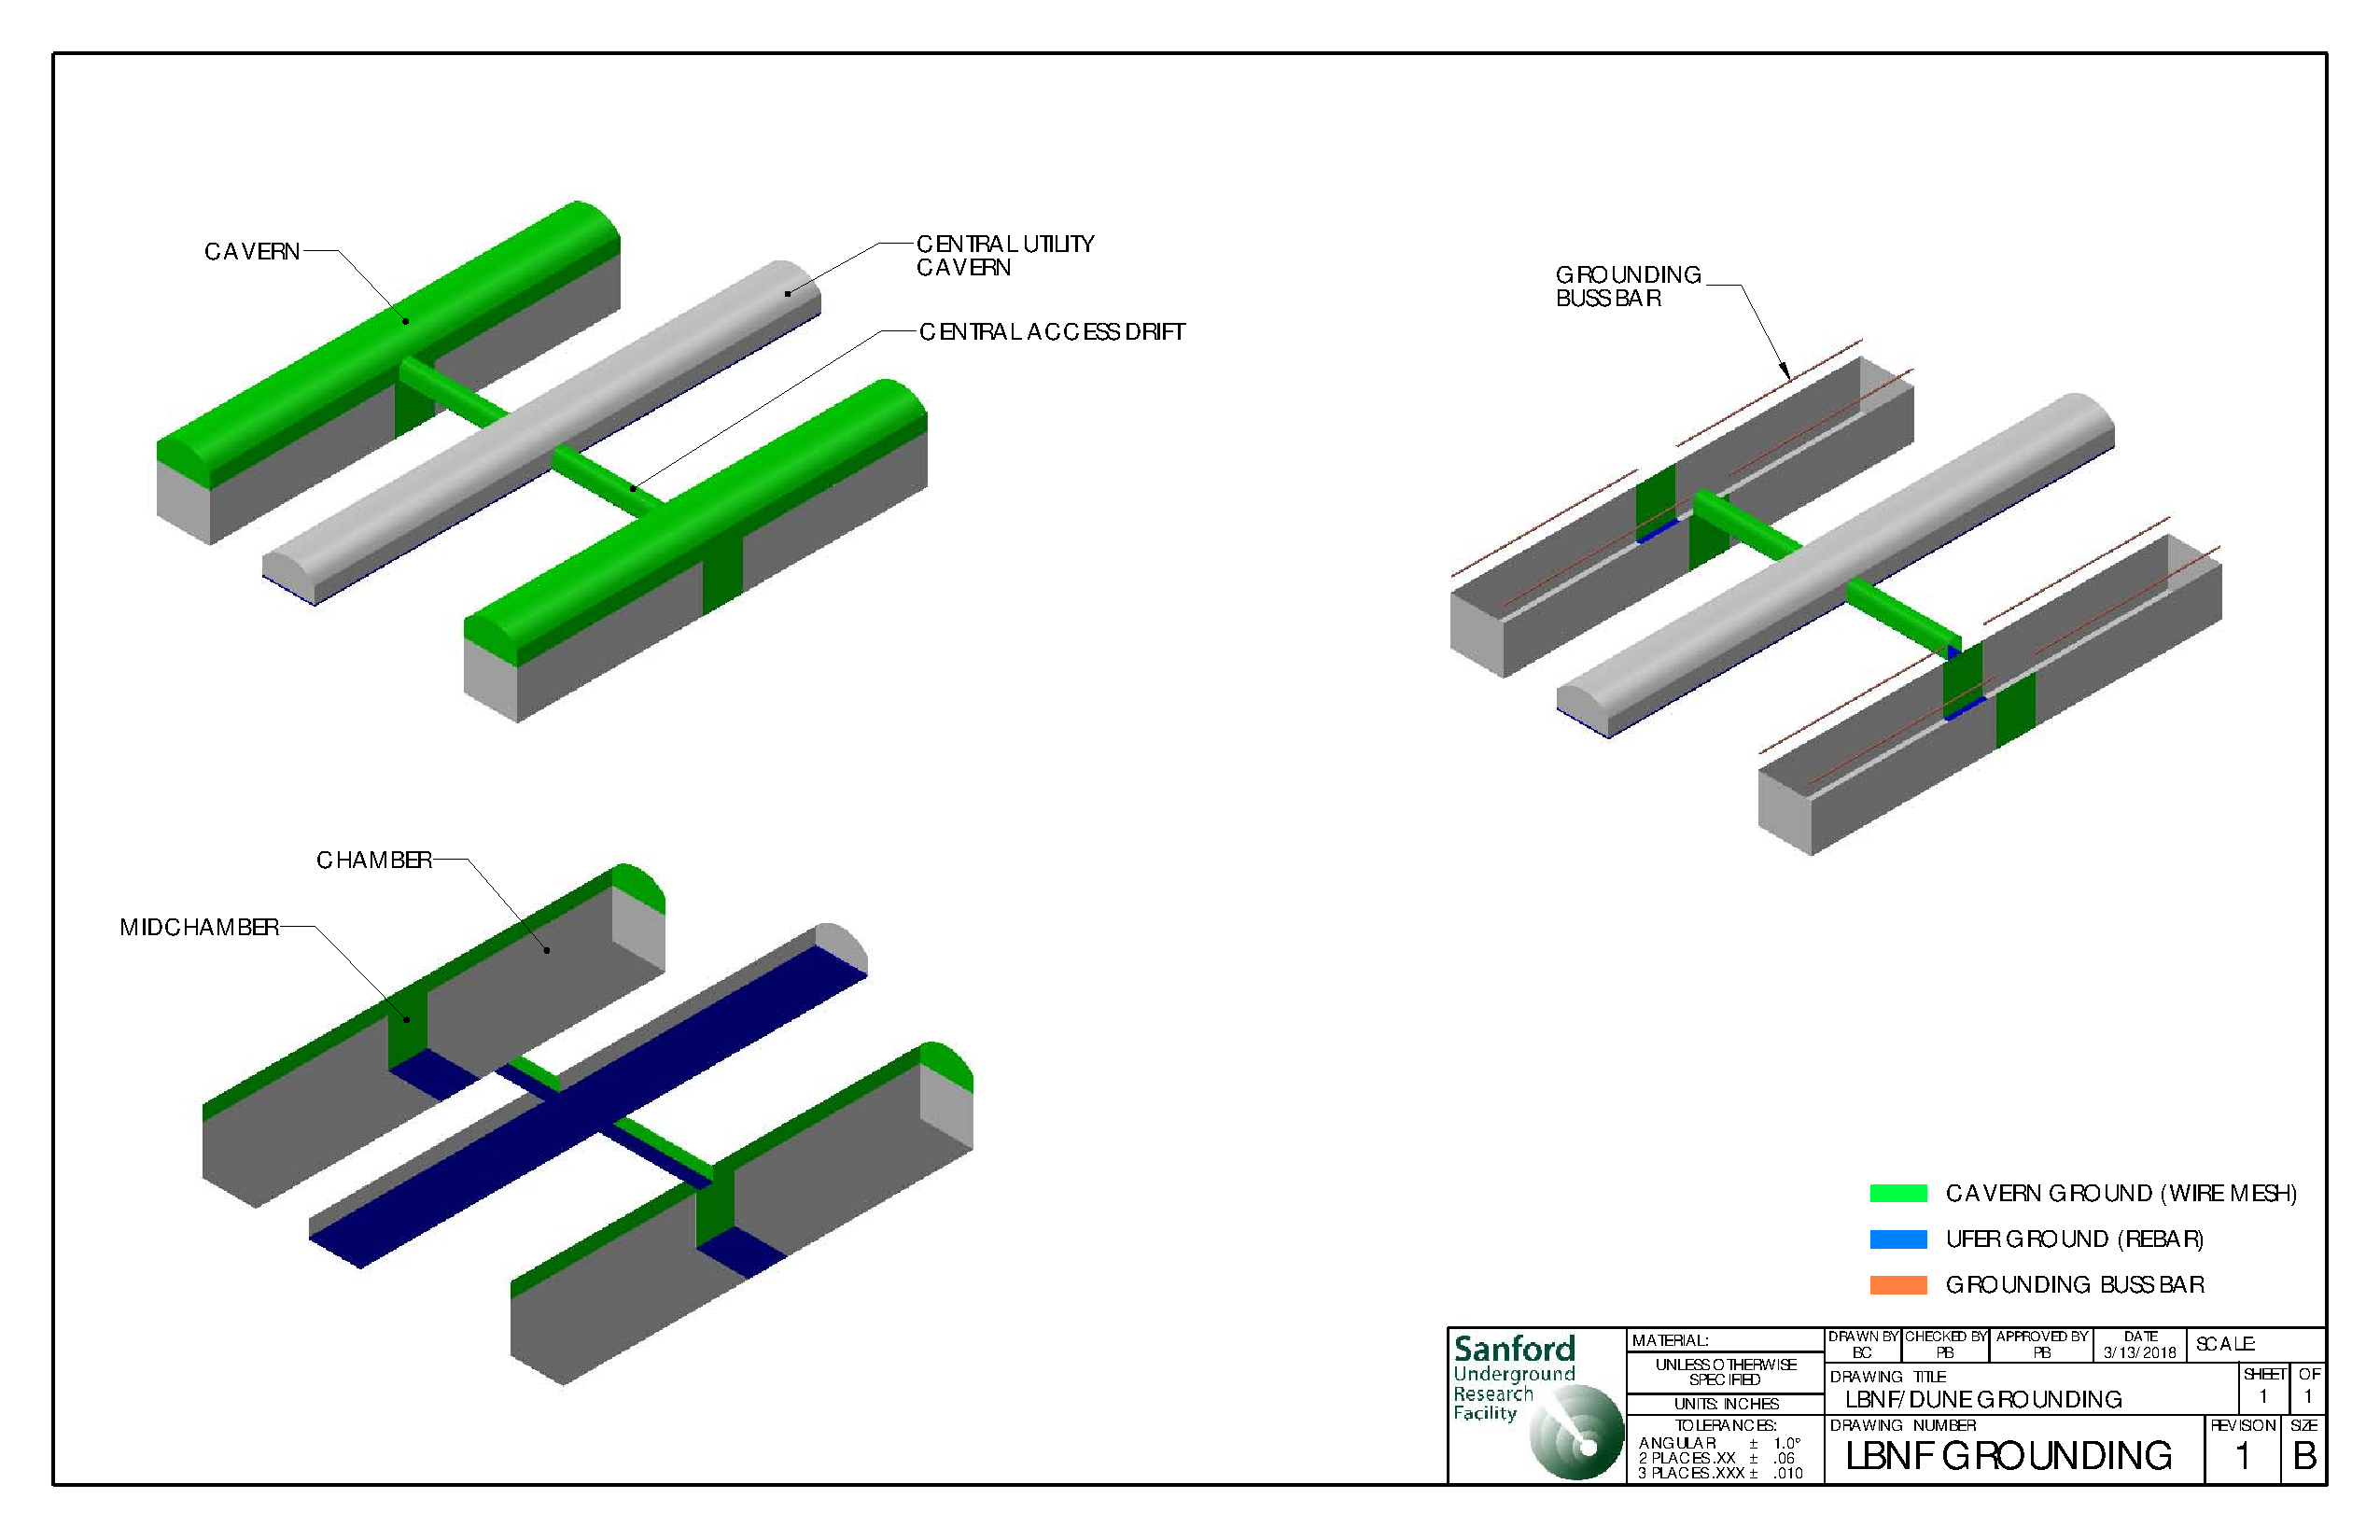
\includegraphics[width=0.85\textwidth]{SURF_Grounding.pdf}
\end{dunefigure}
Grounding structure definitions include:
\begin{enumerate}
 \item Cavern Ground consisting of overlapping welded wire mesh
   supported by rock bolts and covered with shotcrete. The
   \dword{lbnf}/\dword{dune} Cavern Ground includes all walls and
   crown areas above the 4850 level in the north and south detector
   caverns and their associated central access drifts, as well as tin-plated
   copper bus bars that run the length of the detector vessels
   on each side along the cavern walls and are mounted external to the
   shotcrete.  The Cavern Ground structure
\begin{enumerate}
 \item spans the full length of the cavern from the west end access
   drift entrance through the mid-chamber to the east end access drift
   entrance;
 \item spans the full width of the cavern from the 4850 level sill
   (top of the detector vessels and mid-chamber floor) on both sides
   up and across the crown of the cavern;
 \item includes mid chamber walls to the 4910 level;
 \item includes the east and west end walls of the cavern, from the
   4850 level to the crown.
\end{enumerate}
 \item \dword{ufer} ground consisting of metal rebar embedded in
   concrete floors. The \dword{lbnf}/\dword{dune} \dword{ufer} ground
   system includes the concrete floors in the cavern mid-chambers,
   center access drifts, and central utility cavern. The Cavern and
   \dword{ufer} Grounds will be well bonded electrically to construct
   a single facility ground isolated from detector ground.
 \item Detector Ground consists of the steel containment vessel
   enclosing the cryostat and all metal structures attached to or
   supported by the detector vessel.
\end{enumerate}


To ensure safety, a safety ground with one or more saturable inductors
will be installed between the Detector Ground and the electrically
bonded \dword{ufer} and Cavern Grounds which form the facility ground.
Figure~\ref{fig:dune-grounding_figure} illustrates the use of the
safety ground. The safety ground inductors saturate with flux under
low-frequency high currents and present minimal impedance to that
current.  Thus, an AC power fault current would be shunted to the
facility ground and provide a safe grounding design. At higher
frequencies and lower currents, such as coupled noise currents, the
inductor provides an impedance to this current, restricting its flow
between grounded metal structures. The desired total impedance between
the detector ground structure and the Cavern/\dword{ufer} ground
structure should be a minimum of \SI{10}{Ohms} at \SI{10}{MHz}.

\begin{dunefigure}[Simplified detector grounding]{fig:dune-grounding_figure}
  {Simplified detector grounding scheme.}
  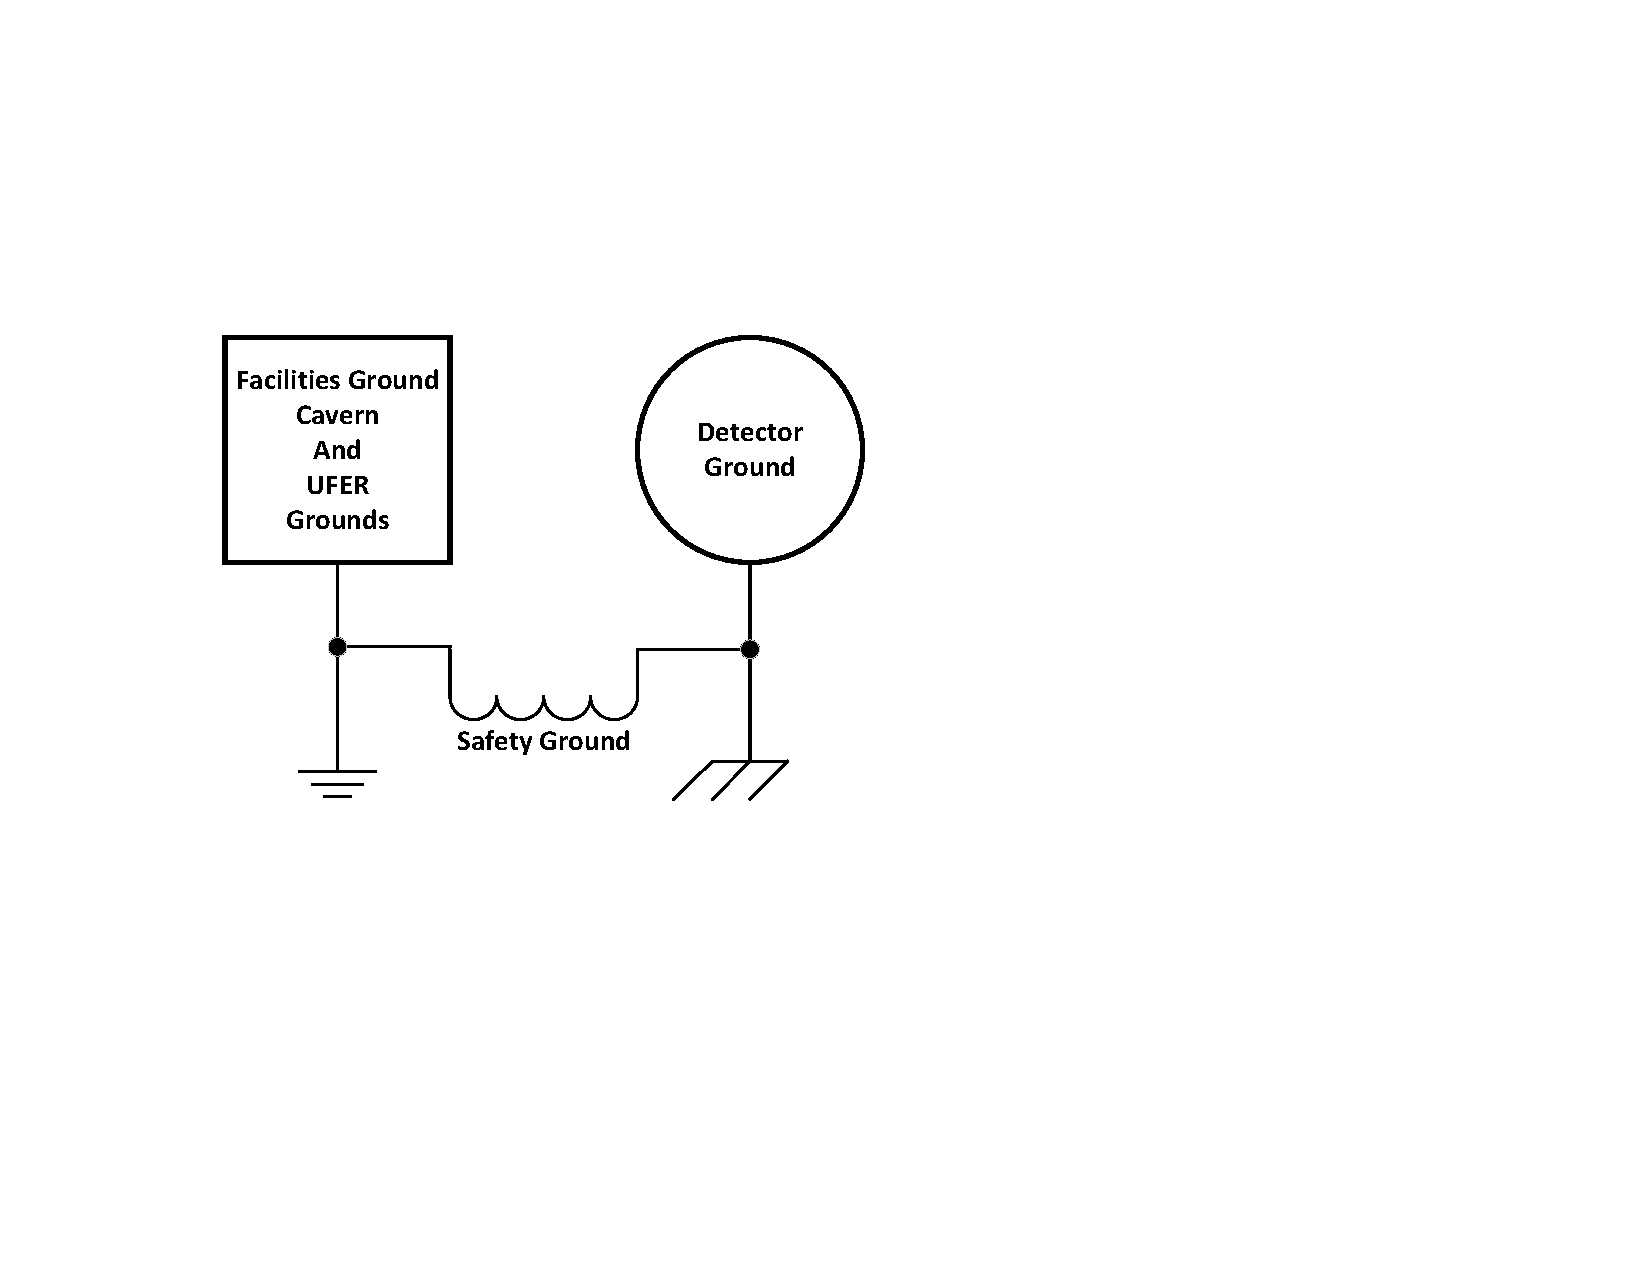
\includegraphics[width=0.5\textwidth]{Simplified_Grounding_Figure.pdf}
\end{dunefigure}

As stated above, the Detector Ground exists only in the area of the
steel containment vessel enclosing the cryostat and all metal
structures attached to or supported by the detector vessel.  All
signal cables which run between the detector and the DAQ Underground
Processing Room in the Central Utilities Chamber will be fiber optic.
All connections to the cryogenic plant which will be on the facility
ground will be isolated from the cryostat with dielectric breaks.  A
conceptual drawing showing the isolation of the cryostat is presented
below in Figure~\ref{fig:dune-grounding_scheme}

\begin{dunefigure}[Detector grounding schematic]{fig:dune-grounding_scheme}
  {Schematic of detector grounding system.}
  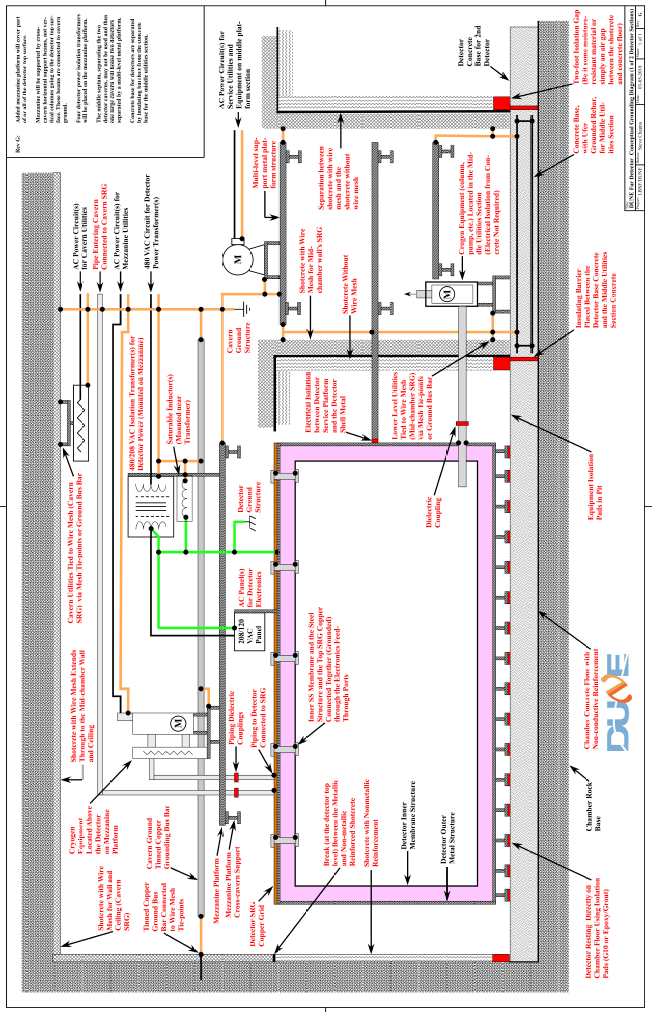
\includegraphics[width=0.75\textwidth]{DUNE_Grounding_figure_vertical.PNG}
\end{dunefigure}

The construction of the facility ground provides a low impedance path
for return currents of the facility services, such as cryogenic pumps,
and noise coupling from facility services will be greatly reduced or
eliminated.  The experiment has also been carefully designed such that
facility return currents will not flow under the cryostats.

The cryostat itself is treated as a Faraday cage.  Any connections
coming from facilities outside of actual detector electronics are
electrically isolated from the cryostat.  For detector electronics,
specific rules for signal and power cables penetrating the cryostat
are given in EDMS 2095958.





\section{Detector Power}
\label{sec:fdsp-coord-faci-power}

The DUNE detectors are constrained in both size and power consumption.
Requirements were given to conventional facilities and limits were set
on both the size of the cavern excavation, cooling capabilities and
the power consumption of the electronics. DUNE experiments must stay
within established power requirements.

The conventional facilities will supply a 1000 KVA transformer for
each cavern.  Each cavern will host two DUNE detectors.  Power from
this initial transformer will be de-rated with no more than 75 percent
of total power available at the electrical distribution panels.  We
plan for a maximum consumption of 360 KW per detector.

The cold electronics readout dissipates an estimated 306 W per
APA. The LV power supplies have a controller which adds approximately
35 W per APA and supplies have an efficiency of approximately 85
percent. This adds up to about 400 Watts per APA, or a total load of
60 KW per detector module. The APA wire-bias power supplies have a
maximum load of 465 W per set of six APAs, for a total budget of
around 12 KW. Cooling fans and heaters near the feedthroughs will use
a nominal amount of power, so the overall power budget for cold
electronics is expected to be less than 75 KW.

The PDS electronics are based on the Mu2e electronics and estimate a
total power budget of approximately 6 KW. DUNE plans a power budget of
8 KW due to cable drops and power supply inefficiencies.  The PDS
electronics present a significantly lower power load than the
alternate solution, used in ProtoDUNE-SP.  ProtoDUNE-SP used SSP
modules which would represent a power load of approximately 72 KW per
detector module.

Each of the approximately 80 detector racks will have fan units,
Ethernet switches, rack protection, and slow controls modules, adding
a load of about 500 W per rack, for a total of 40 KW.

Twenty-five racks are reserved for cryogenics instrumentation with a
per-rack load conservatively estimated at 2 KW, for a total of 50 KW.
The SP detector module will thus use an estimated 173 KW of power. The
higher-load SSP alternative for the PDS would increase this to 237
KW. This higher estimate represents approximately 67 percent of our
available power. The Dual Phase electronics estimate is approximately
160 KW and also fits well within the planned maximum of 360 KW.

For the SP detector, the power will be largely distributed to a number
of detector racks which will sit on a detector rack mezzanine above
the cryostat.  Each of the racks will receive a 30-amp 120-volt
service and there will be a maximum of 80 racks.

The other area where DUNE requires power underground is in the DAQ
room.  There the power budget is determined by the available 750 KVA
transformer.  The available power must be de-rated to 80 percent at
the electrical distribution panel and another 80 percent for equipment
efficiency.  Thus, 480 KW of power will be distributed to a maximum of
60 racks.  Each water-cooled rack will have approximately 8 KW
available for computing power.


\section{Data Fibers}
\label{sec:fdsp-coord-faci-fibers}


The \dword{dune} experiment requires a number of fiber optic pairs to
run between the surface and the 4850 level.  A total of 96 fiber
pairs, which includes both \dword{dune} and \dword{lbnf} needs, will
be supplied through redundant paths with bundles of 96 pairs coming
down both the Ross and Yates shafts.  The individual fibers are
specified to allow for transmission of 100 Gbps.  A schematic view of
fiber path from surface to underground is shown in
Figure~\ref{fig:dune-fiber_path}.
\begin{dunefigure}[Detector fiber path]{fig:dune-fiber_path}
  {Schematic of detector fiber path.}
  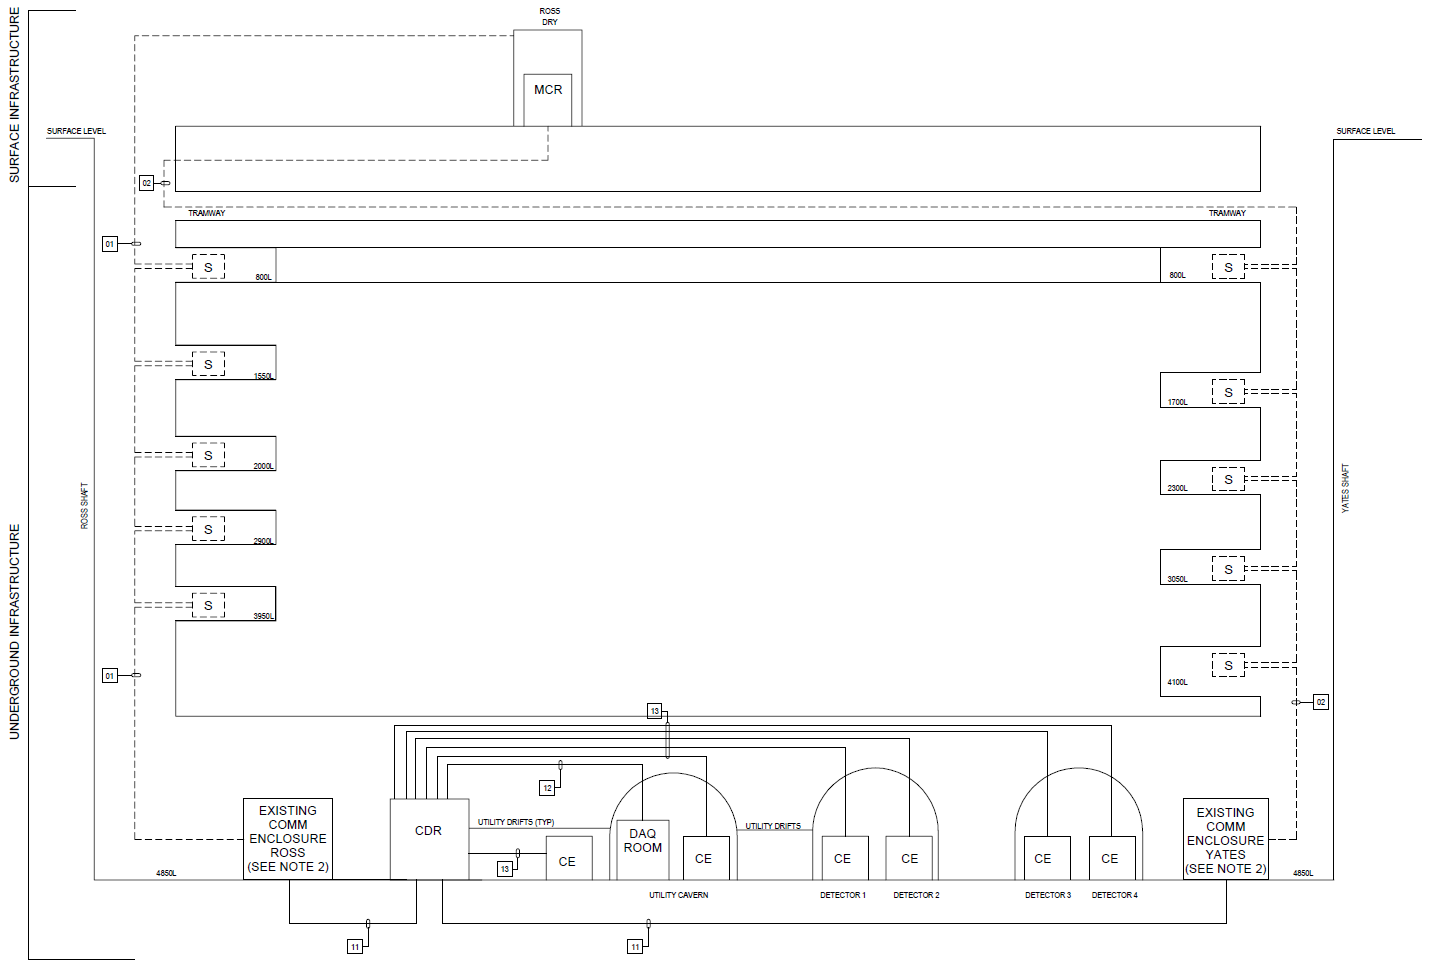
\includegraphics[width=0.85\textwidth]{Fiber_path.PNG}
\end{dunefigure}

The redundant fiber cable runs of 96 fiber pairs are received in
existing communications enclosures at the 4850L entrances of the Ross
and Yates shafts.  The two 96 fiber pair bundles are next routed to a
Communication Distribution Room (CDR).  The fibers will be received
and terminated in an optical fiber rack. Two additional network racks
will be used to route the fiber data between the surface and
underground.

The plan is to use only the Ross shaft set of 96 fiber pairs with the
Yates set being redundant.  The network switches will allow for
switchover in case of catastrophic failure of fibers in the Ross
shaft.  Plans are being formed to periodically test the redundant
Yates path and verify its viability.

From the CDR, fibers designated for Far Site Conventional Facilities
(FSCF) are routed to provide general network connections to the
detector caverns, central utility cavern and the underground DAQ room.

A total of 96 fiber pairs are routed to the underground DAQ room for
use by the DUNE experiment and LBNF. The fibers are reserved as
follows:
\begin{itemize}
  \item 15 pairs for DUNE data per detector-total 60 pairs
\item 1 pair for slow controls per detector-total 4 pairs
\item 2 pairs reserved for \dword{gps}
\item 6 pairs for FSCF
\item 4 pairs for LAr cryogenics
  \item 4 pairs for LN2 cryogenics
\end{itemize}

The set of reserved fiber pairs total to 80, the remaining 10 pairs
are available for assignment or as spares.


\section{Central Utility Cavern Control and DAQ Rooms}
\label{sec:fdsp-coord-cuc-daq}

The \dword{cuc} contains various cryogenic equipment and the
\dword{daq} and Control Room for the \dword{dune} experiment.  The
cryogenic system and areas are described in
Section~\ref{sec:fdsp-coord-cryogenics} . Both the control and DAQ
rooms are in the west end of the \dword{cuc} (see
Figure~\ref{fig:dune-cuc}).
\begin{dunefigure}[DAQ and control rooms in CUC]{fig:dune-cuc}
  {Location of underground DAQ and control rooms in the CUC.}
  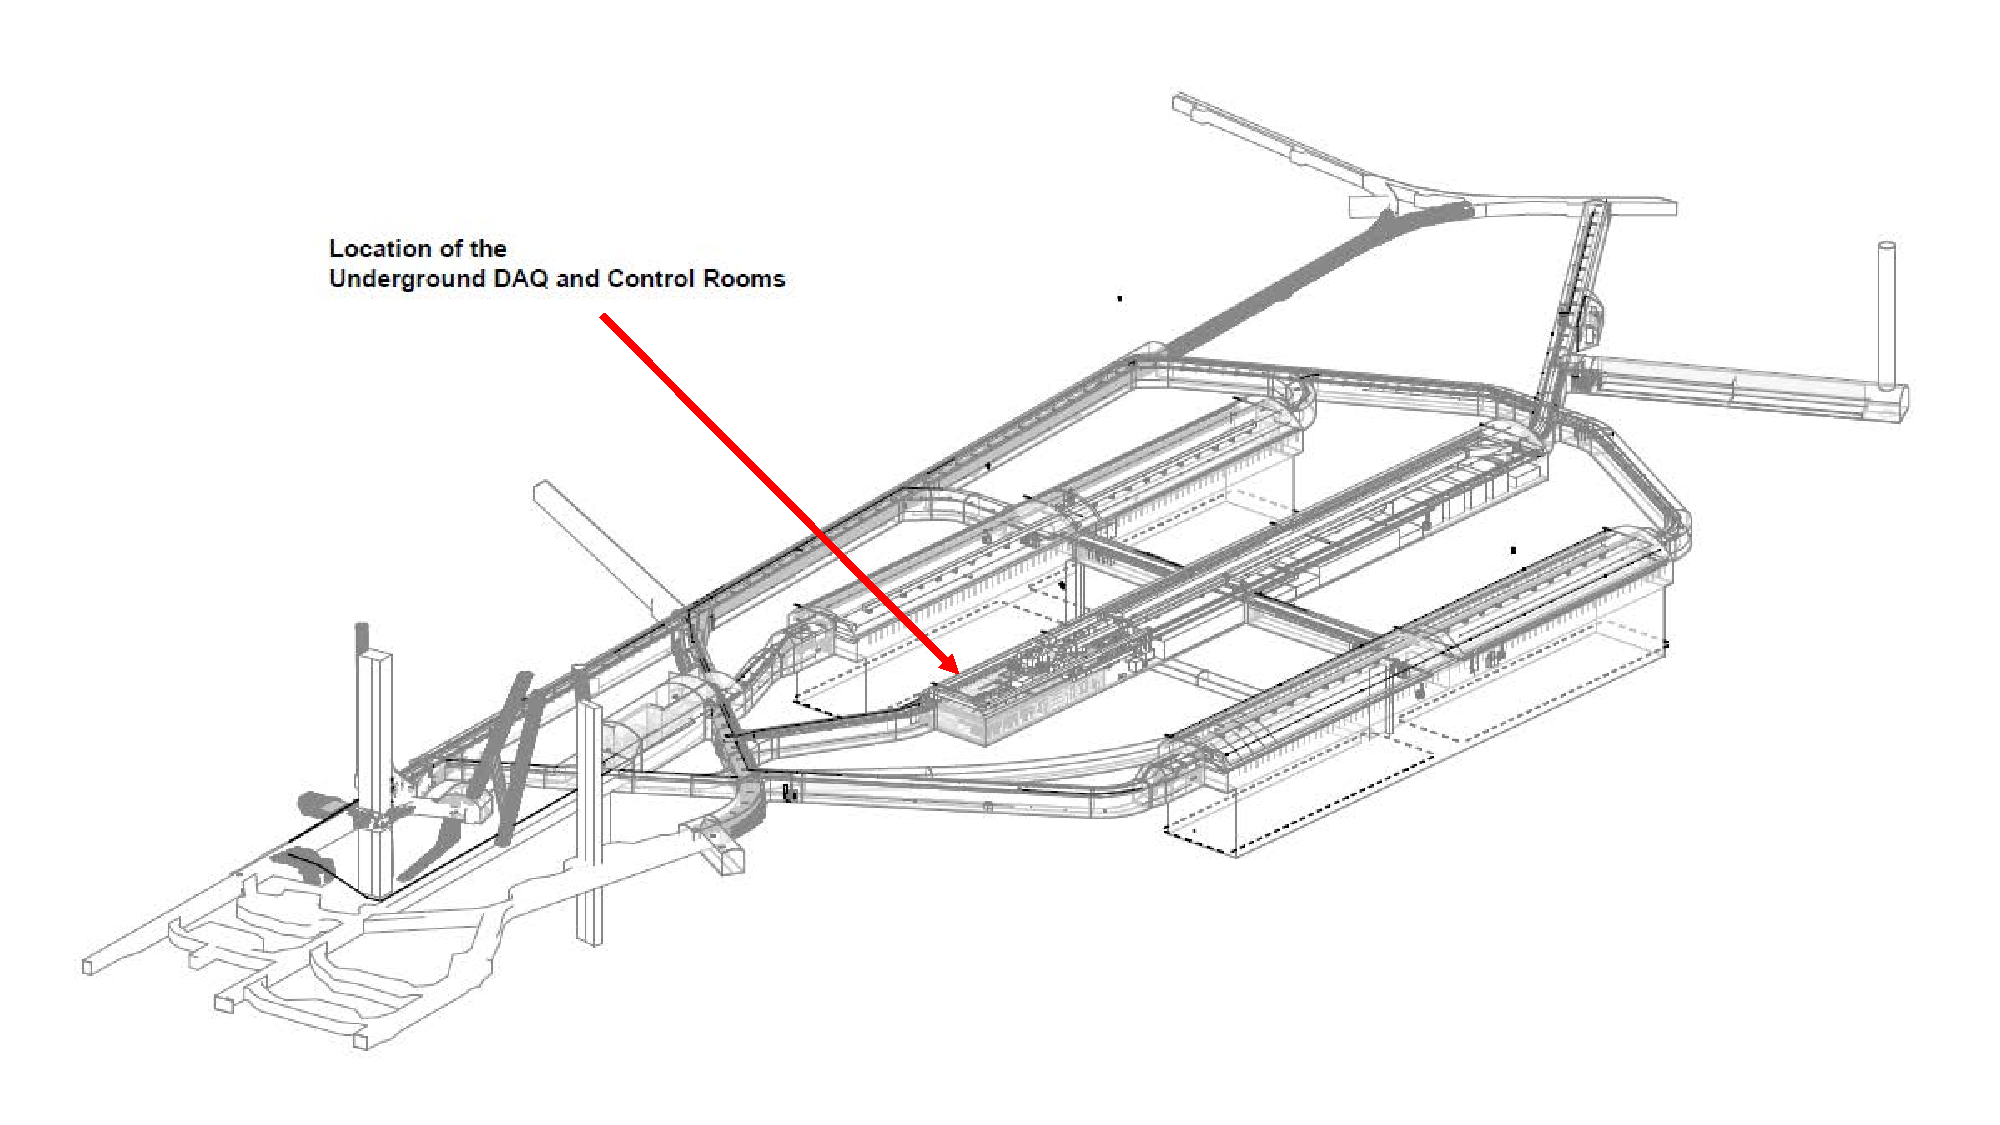
\includegraphics[width=0.85\textwidth]{Location_Underground_DAQ_Control_Rooms.pdf}
\end{dunefigure}
\begin{dunefigure}[DAQ and control rooms]{fig:dune-daq}
  {Underground DAQ and control rooms layout.}
  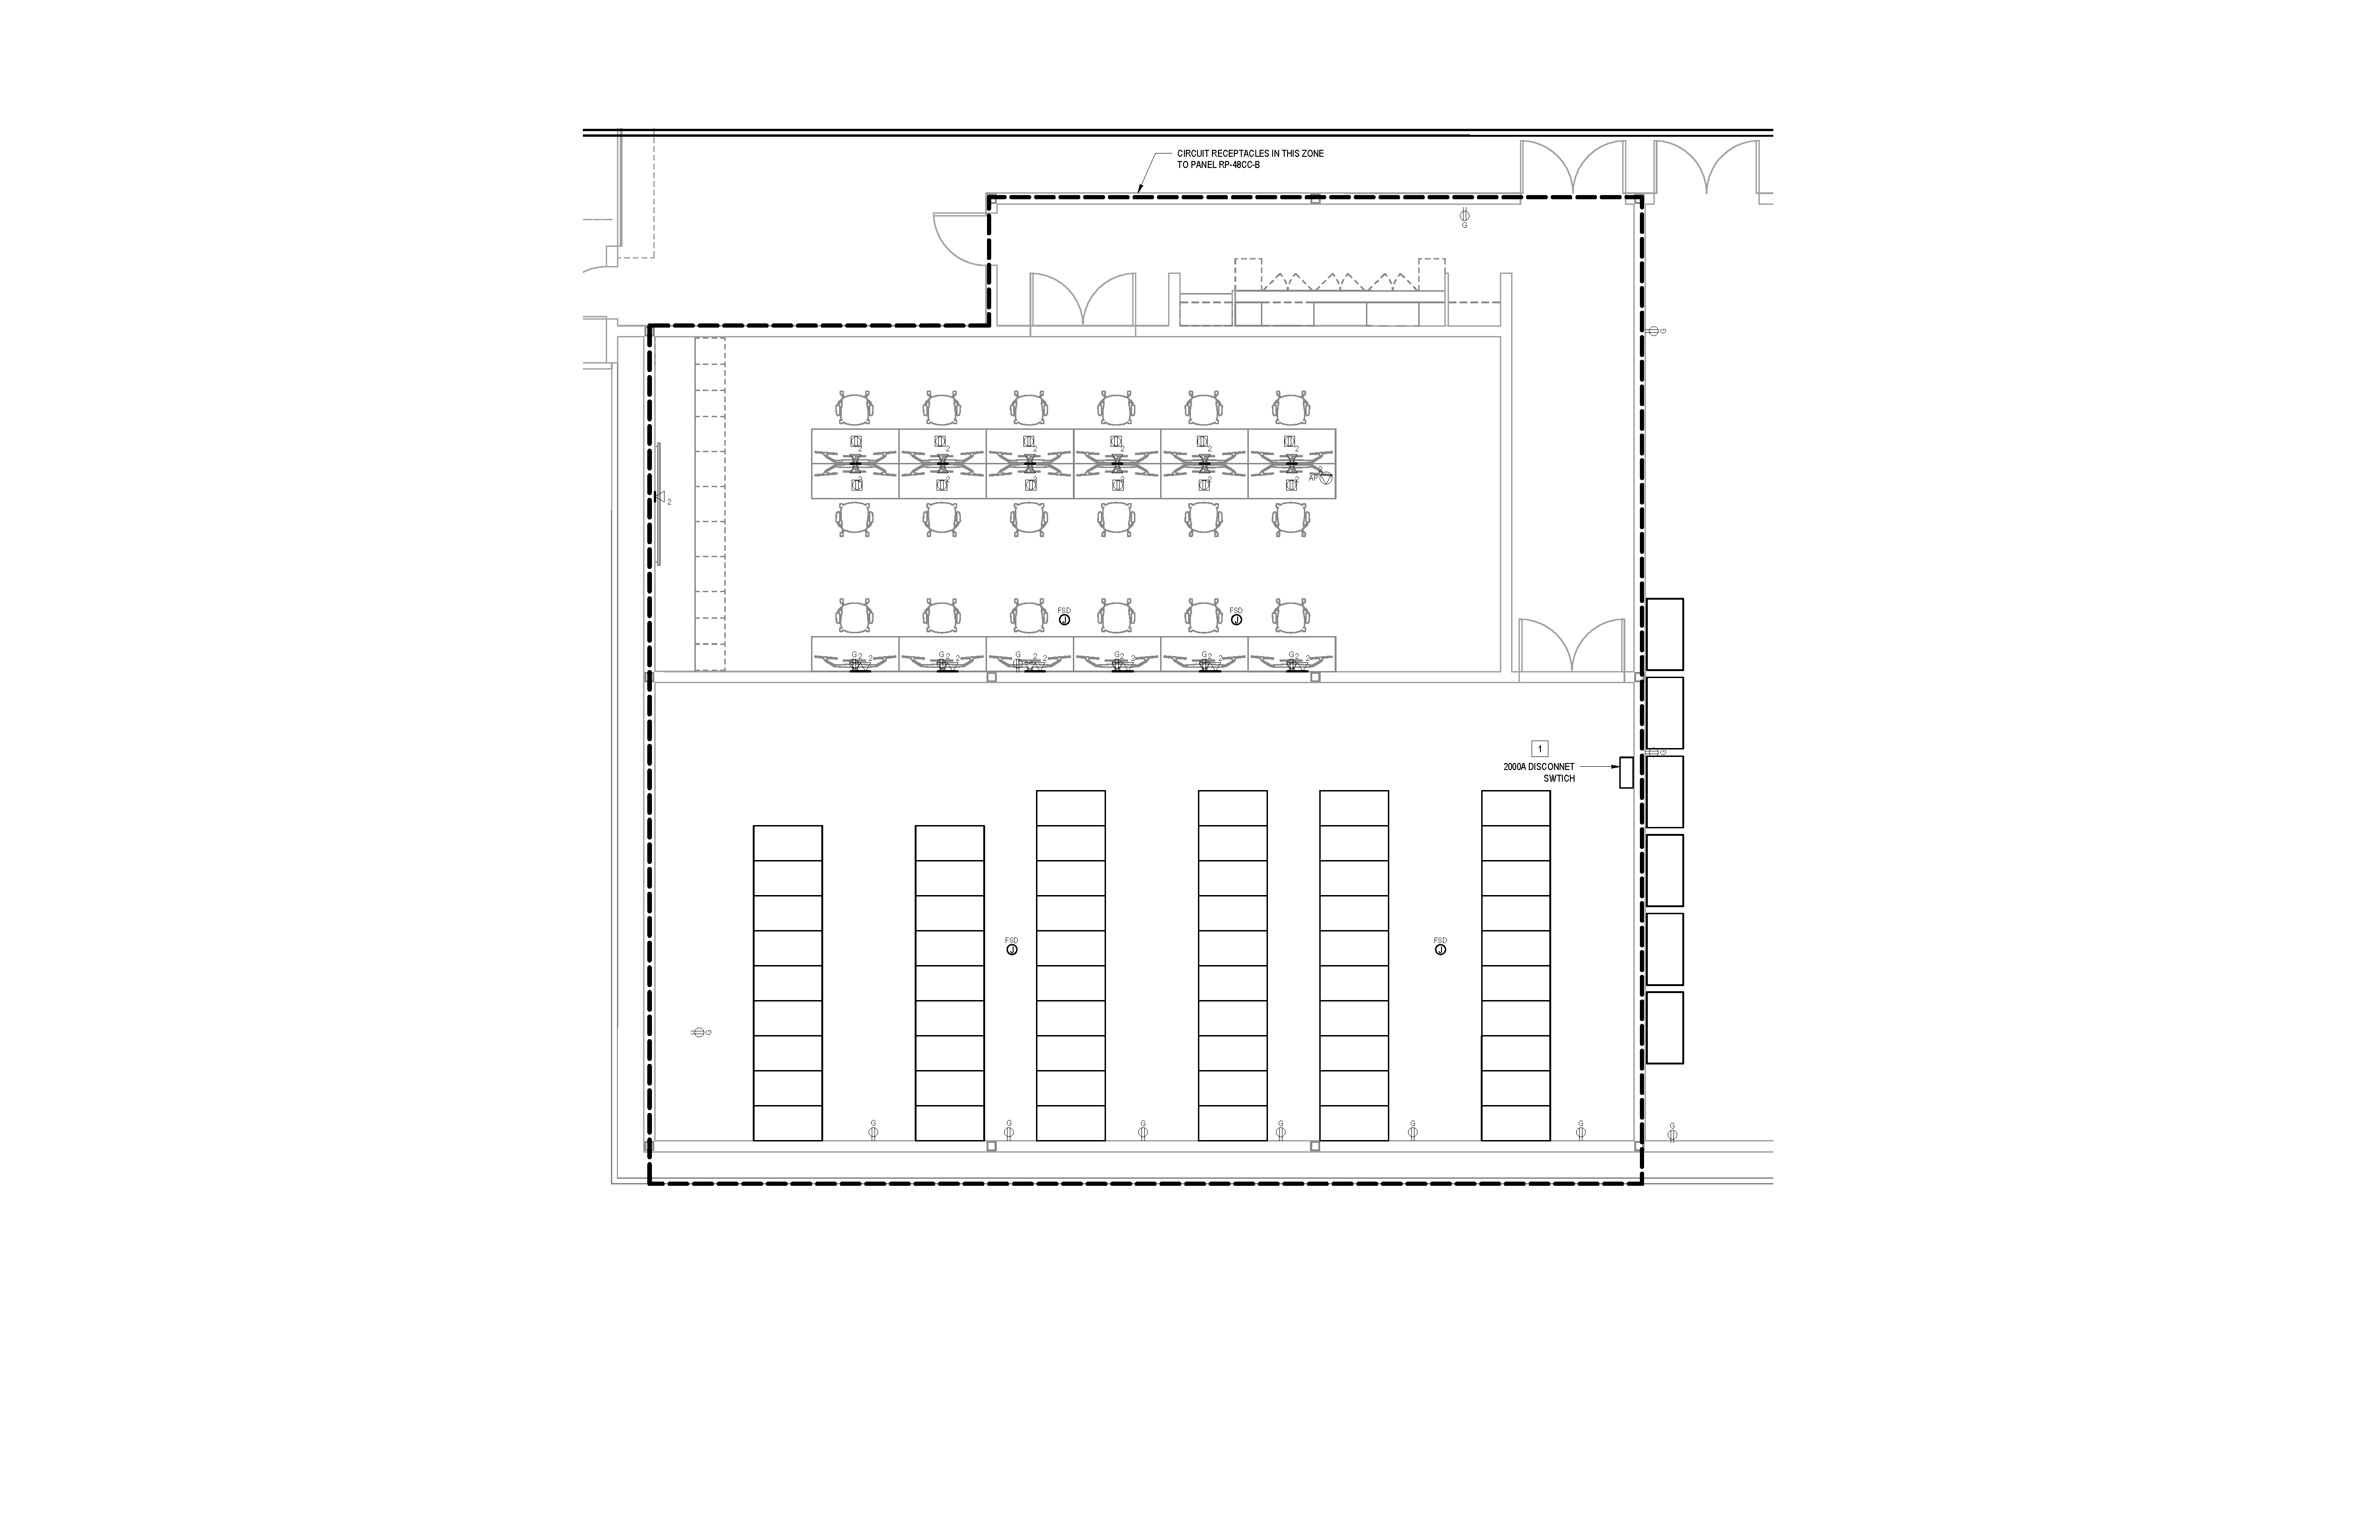
\includegraphics[width=0.85\textwidth]{Preliminary_Layout_DAQ_Control_Rooms.pdf}
\end{dunefigure}


The Control Room is an underground space of approximately 18 x 48 feet
and serves multiple purposes.  It provides a meeting or work space
where five to ten people can sit with laptops during system
commissioning.  It is not truly a control room from which the
experiment will be run.  The DUNE experiment will have a remote
control room located at Fermilab's main campus.  Personnel involved in
commissioning the experiment are expected to be working in the
Detector Caverns, not the CUC.  If DAQ equipment need to be serviced,
an experience and trained group of technicians will be able to work
with remote collaborators to address issues in the DAQ room.

Figure~\ref{fig:dune-daq} shows the layout and suggested outfitting of
the rooms. Additionally, the Control Room provides the required
workstation for monitoring of Fire and Life Safety, and the building
management system.  These are facility services for which DUNE is not
directly responsible for, however, the experiment will need to
interface with these systems.  One example of this interface would be
the reporting of any smoke detected within a detector rack.

Lastly, the cryogenic team requires a space allocation within the
Control Room of two racks and two work benches for the technicians who
monitor the cryogenic systems.  This space is needed only during
commissioning with remote operation to follow.
       
The \dword{daq} room is approximately 26 x 56 square feet and will
contain between 52 to 60 racks that will be used for fiber optic cable
distribution, networking, \dword{dune} \dword{daq} and two or three
racks for conventional facilities.  The current design, shown in
Figure~\ref{fig:dune-DAQ_layout}, shows a total of 60 racks are
possible.
\begin{dunefigure}[DAQ room layout]{fig:dune-DAQ_layout}
  {Proposed rack layput in DAQ room.}
  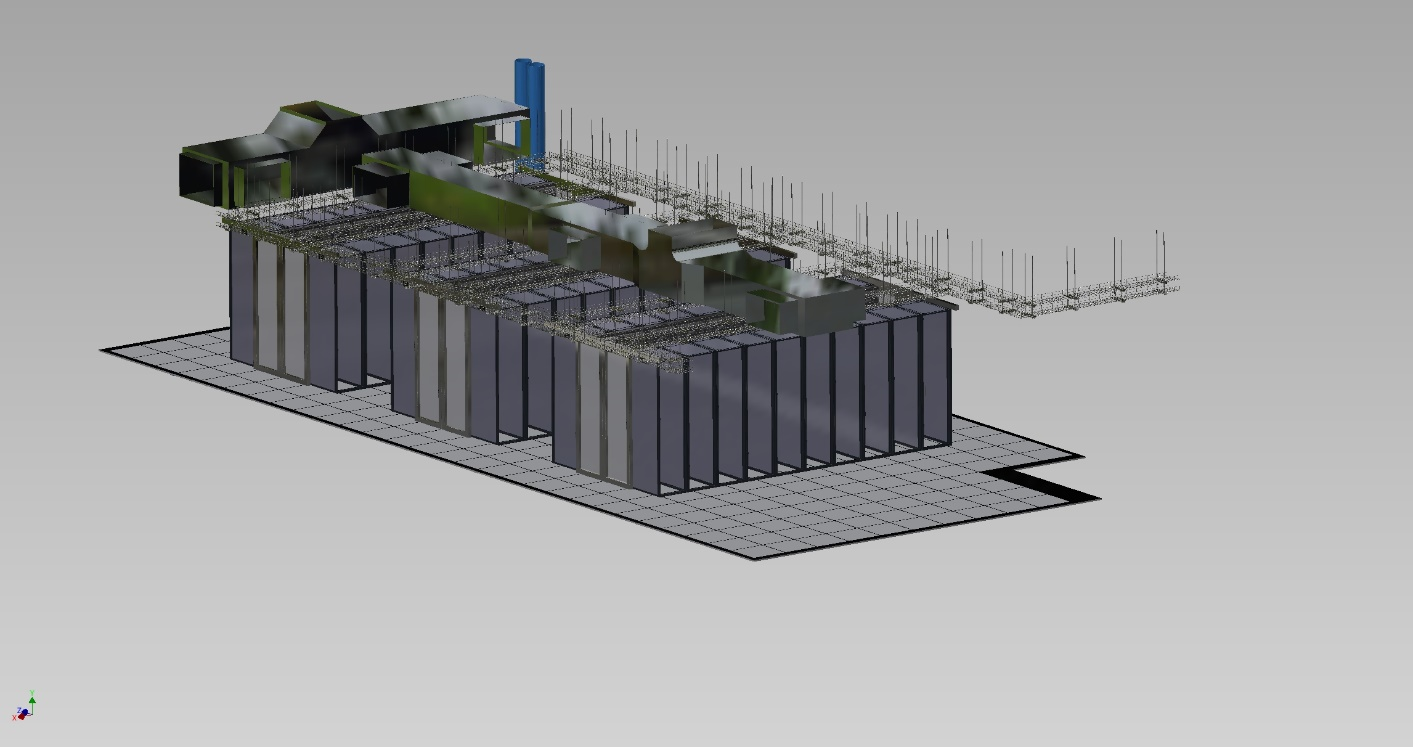
\includegraphics[width=0.85\textwidth]{Prop_DAQ_room_layout.png}
\end{dunefigure}
  

A quantity of 48 racks are reserved exclusively for \dword{daq}.  Two
additional racks are required for optical fiber distribution and
network connection to the surface.

Conventional facilities will supply the \dword{daq} room with cooling
water, an 18~inch raised floor, lighting, HVAC, dry fire protection
and dedicated 750kVA transformer.  \Dword{tc} will be responsible for
the final outfitting and layout of the room.  This includes the layout
and installation of water cooled racks, design and installation of
piping that carries cooling water to the racks, the AC power
distribution to the racks and installation of cable trays.

\section{Surface Rooms}
\label{sec:fdsp-coord-surf-rooms}

The \dword{dune} experiment requires space on the surface for a small
number of DAQ, networking, and fiber optic distribution racks.  Space
is also allocated for cryogenics.  The surface cryogen building and
operations will be described in section
Section~\ref{sec:fdsp-coord-cryogenics}

The \dword{daq} consortium requires a surface computer room with eight
racks and a minimum of 50kVA of power.  DAQ also requires connection
to the optical fibers running to the 4850L via the Ross and Yates
shafts as well as to the Energy Sciences Network (ESnet).

The surface DAQ, networking equipment, and fiber distribution racks
will be placed in a new Main Communications Room (MCR) in Ross Dry
Building.  The MCR is approximately 628 square feet and will be
completed as part of the LBNF project, with seven racks installed for
the conventional facilities and space allocated for eight racks
provided by the experiment.  The seven racks allocated for
conventional facilities will include networking and fiber optic
distribution.  The eight racks allocated to the experiment will
contain computer servers, disk buffer and some network connections.
Power and cooling will be provided as part of the LBNF project.
\begin{dunefigure}[Surface rooms layout]{fig:dune-surface_layout}
  {Ross area surface rooms layout.}
  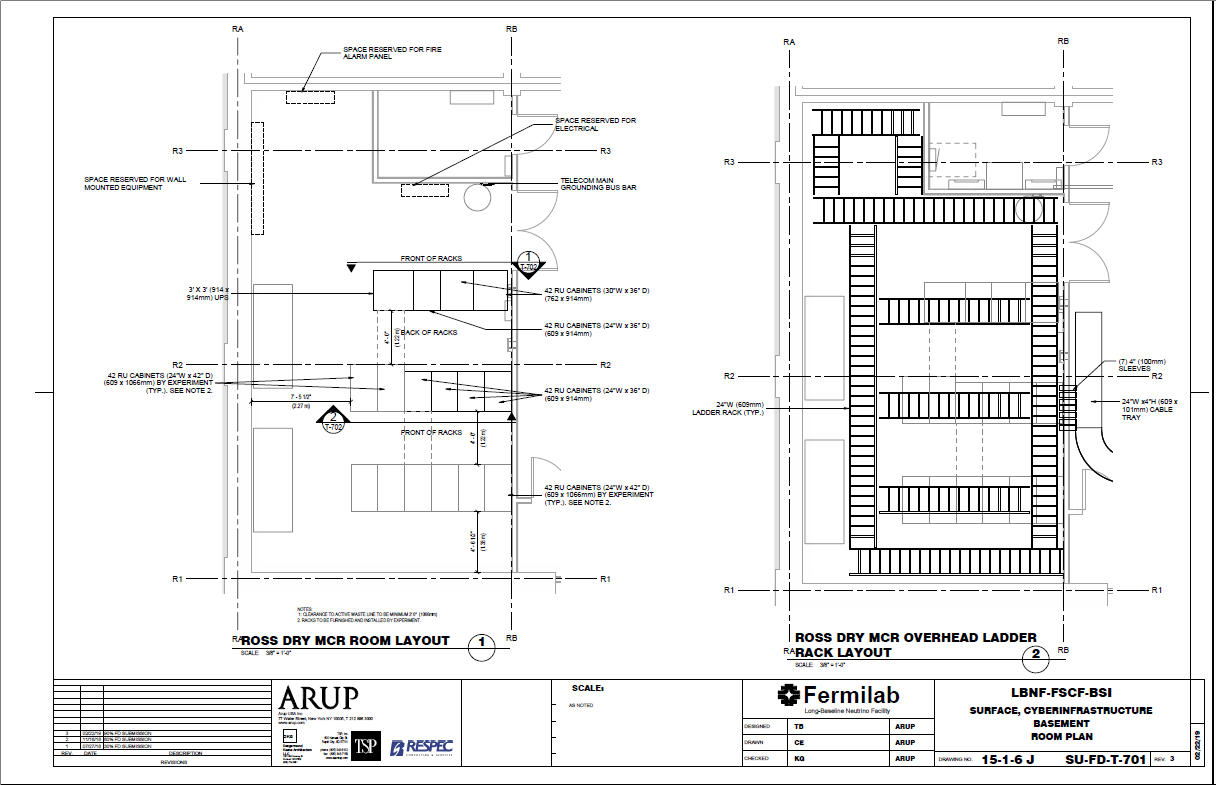
\includegraphics[width=0.85\textwidth]{Surface_rooms_layout.png}
\end{dunefigure}


\section{\dword{dune} Detector Safety System}
\label{sec:fdsp-coord-det-safety}


The \dword{dune} Detector Safety System (\dword{ddss}) functions to
protect experimental equipment.  The system must detect abnormal and
potentially harmful operating conditions.  It must recognize when
conditions are not within the bounds of normal operating parameters
and automatically take pre-defined protective actions to protect
equipment.  Protective actions are hardware or Programmable Logic
Controller(\dword{plc}) driven.

Dune Technical Coordination must work with the detectors to identify
equipment hazards and ensure that harmful operating conditions can be
detected and mitigated.  These hazards include smoke detected in
racks, leak(s) detected in water cooling areas, ODH detection, a drop
in the cryostat LAr liquid level, laser or radiation hazards in
calibration systems, over or under voltage conditions, and others to
be determined.  Some hazards will be unique to the actual detector
being implemented.

It is also noted that the \dword{ddss} will provide input to the 4850L
Fire Alarm System.  The 4850L Fire Alarm System will provide life
safety and play an integral role in detecting and responding to an
event as well as notifying occupants and emergency responders.  This
system is the responsibility of the host lab and South Dakota Science
and Technology Authority (SDSTA).  The Fire Alarm System is described
in the BSI Design in Support of LBNF Far Site Conventional Facilities
-- 90\% Fire and Safety Report and can be found in EDMS-2093229. The
4850L Fire Alarm System is connected to the surface Incident Command
vault in the 2nd floor of the Yates Administration building. Limits on
the number of occupants and egress paths are discussed. The table of
triggering inputs and Fire Alarm Sequence of Operation is documented
in the set of BSI Underground Electrical drawings, sheet U1-FD-E-308
which is also found in EDMS-2093229. The experiment will be adding a
list of initiating inputs, such as smoke detected in electronic racks
or water leaks detected in the DAQ room to this sheet as designs reach
a higher level of maturity. For additional information regarding the
facility safety systems see Section~\ref{sec:fdsp-coord-host_facility_services}.
 
The \dword{ddss} must communicate to the \dword{dune} slow controls
system as well as the 4850L Fire Alarm System.  The \dword{dune} slow
controls system has the task of monitoring and recording detector
status.  Working together through communication links, the three
systems will monitor the status of the experiment (Slow Controls),
protect equipment (\dword{ddss})and provide life safety (4850L Fire
Alarm System). Figure~\ref{fig:dune-DDSS} indicates how these systems
interact, with a few illustrated examples.
\begin{dunefigure}[\dword{ddss}]{fig:dune-DDSS}
  {\dword{ddss} block diagram.}
  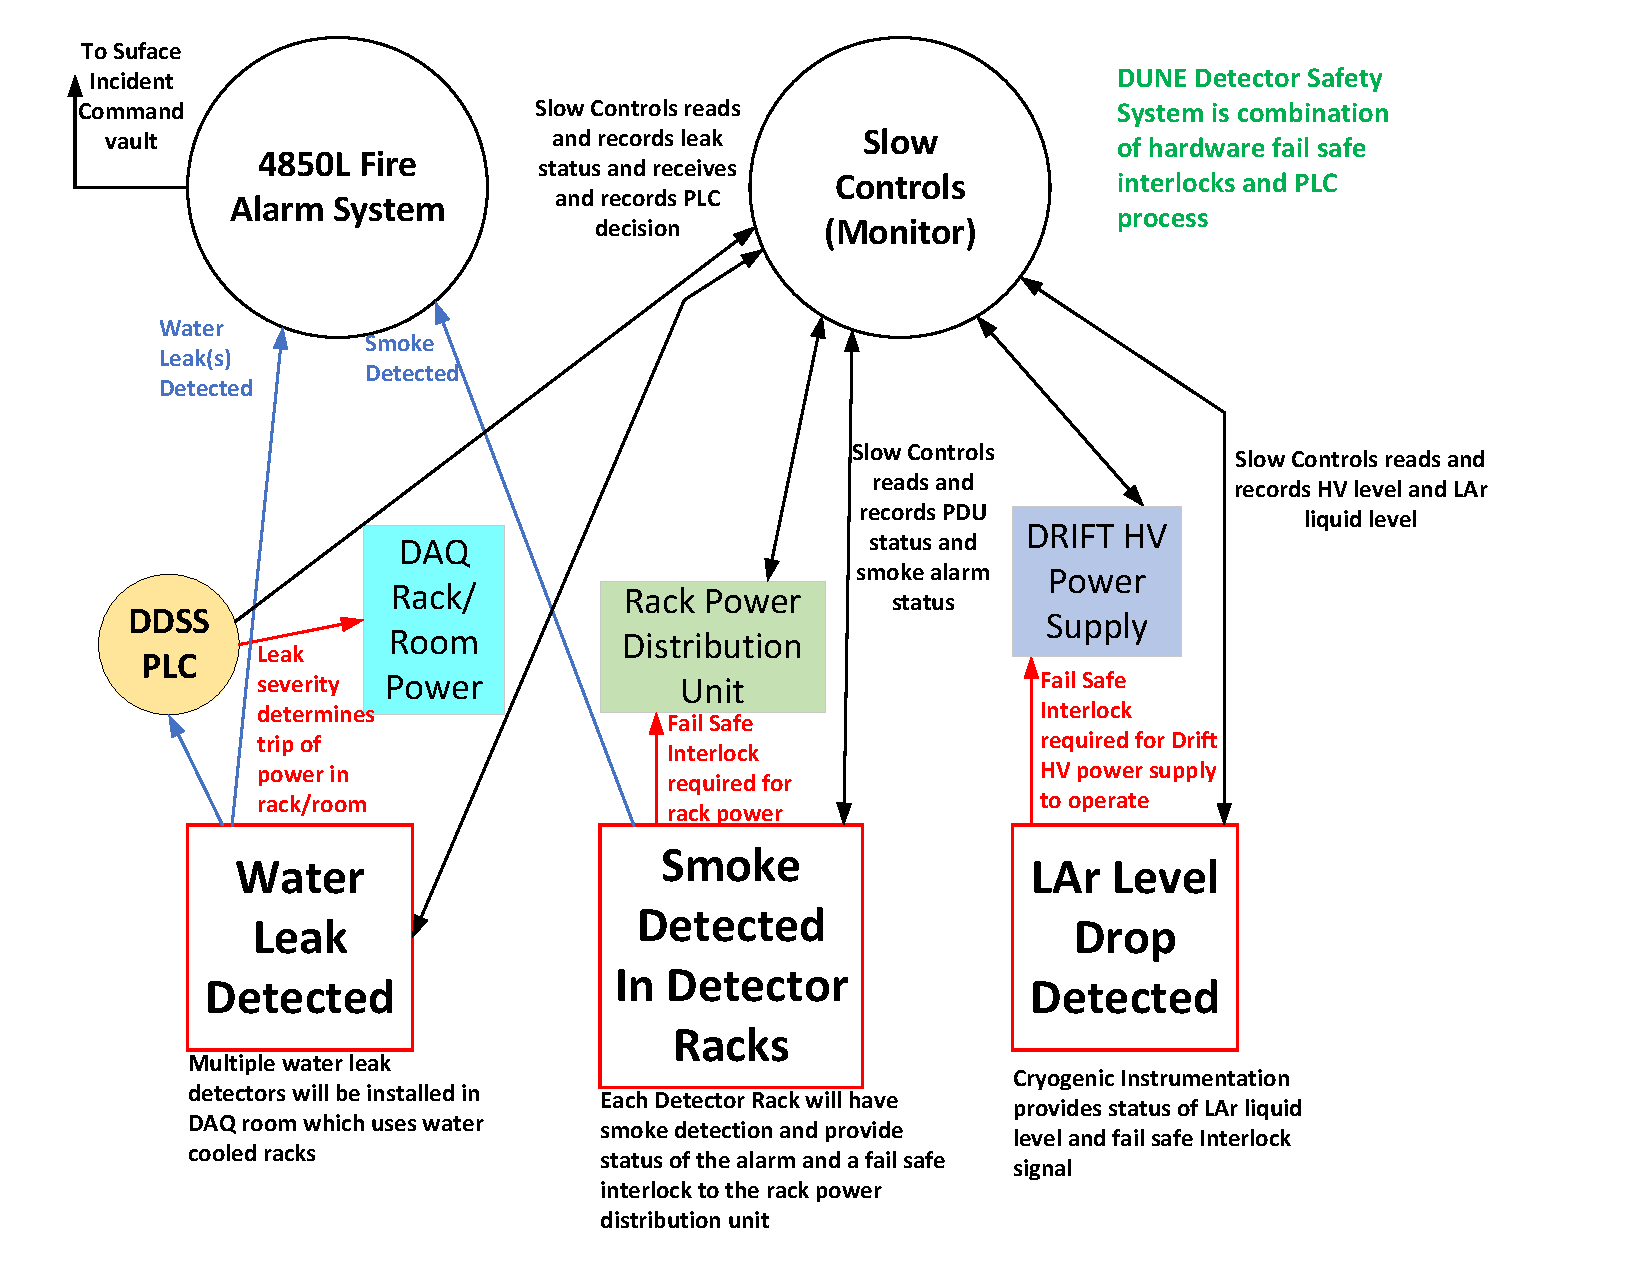
\includegraphics[width=0.85\textwidth]{DDSS_Block_Diagram.pdf}
\end{dunefigure}


The \dword{ddss} will be implemented through hardware interlocks and a
\dword{plc}.  The selection of the \dword{plc} hardware platform is
still an open decision.  Listed below are some of the general
\dword{dune} experimental conditions that require intervention of the
\dword{ddss}:
\begin{enumerate}
 \item A drop in the \dword{lar} level.  This condition requires a hardware
   interlock on the liquid level.  If the level drops below a
   pre-determined level, the drift high voltage must automatically be 
   shut off to prevent equipment damage due to high voltage discharge.  Slow controls would be
   alerted through normal monitoring and record the status of the detector.
 \item Smoke or a temperature/humidity increase above normal operating
   levels. This could be detected inside a rack or near an instrumented
   feedthrough.  If any of these conditions are detected, local
   power must be automatically switched off. If smoke is detected, a
   dedicated line will alert 4850L Fire Alarm System.
 \item A water leak detected near energized equipment in the \dword{daq}
   underground data processing room.  Water leak detectors 
   report to the \dword{ddss} \dword{plc} and a decision will be made to either
   issue an alert or immediately shut power down to the room depending
   on the detected magnitude of the leak.  This condition would also be reported
   to the 4850L Fire Alarm System.
\end{enumerate}



%\section{LBNF/SURF Safety System}
%\label{sec:fdsp-coord-surf-safety}

